\documentclass[a4paper,12pt]{article}

\usepackage[margin=2cm]{geometry}
\usepackage[utf8]{inputenc}
\usepackage[english]{babel}
% \usepackage{textcomp}

\usepackage[font={small,it}]{caption}

\usepackage{color}
\usepackage{graphicx}
\usepackage{epstopdf}
\usepackage{amsmath}
\usepackage{amsfonts}
\usepackage{mathtools}
\usepackage{dsfont}
\usepackage{color}
\usepackage{verbatim}
\usepackage[inline]{enumitem}
\usepackage{listings}
\usepackage{wrapfig}
\usepackage{makeidx}
\usepackage{tikz}

\usepackage{cite}
\usepackage{hyperref}
\bibliographystyle{apalike}


\usepackage{kpfonts}


\hypersetup{%
    colorlinks,
    citecolor=black!90!blue!40,
    linkcolor=black!50!blue!90,
    urlcolor=black!50!blue!90
}

\makeindex

\begin{document}

\begin{titlepage}
    \begin{center}
        \vspace*{3cm}
   
        {\ttfamily\LARGE Plasmons in Fractals\par}
        
        \vspace{1.5cm}
        
        {\ttfamily\large\textbf{Tom Westerhout} \par}
        
        \vspace{0.5cm}

        {\ttfamily\textit{Supervisors}: Shengjun Yuan \& Edo van Veen}
        
        \vfill
        
        
        \hbox{\hspace{5.6cm}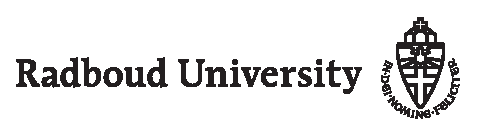
\includegraphics{ru_e_a4_zwart_2014.eps}}
        
        {\ttfamily Theory of Condensed Matter \par}
        {\ttfamily 15 August 2017}

        \vspace{2cm}
        
    \end{center}
\end{titlepage}

\begin{center}
    % GNUPLOT: LaTeX picture with Postscript
\begingroup
  \makeatletter
  \providecommand\color[2][]{%
    \GenericError{(gnuplot) \space\space\space\@spaces}{%
      Package color not loaded in conjunction with
      terminal option `colourtext'%
    }{See the gnuplot documentation for explanation.%
    }{Either use 'blacktext' in gnuplot or load the package
      color.sty in LaTeX.}%
    \renewcommand\color[2][]{}%
  }%
  \providecommand\includegraphics[2][]{%
    \GenericError{(gnuplot) \space\space\space\@spaces}{%
      Package graphicx or graphics not loaded%
    }{See the gnuplot documentation for explanation.%
    }{The gnuplot epslatex terminal needs graphicx.sty or graphics.sty.}%
    \renewcommand\includegraphics[2][]{}%
  }%
  \providecommand\rotatebox[2]{#2}%
  \@ifundefined{ifGPcolor}{%
    \newif\ifGPcolor
    \GPcolortrue
  }{}%
  \@ifundefined{ifGPblacktext}{%
    \newif\ifGPblacktext
    \GPblacktexttrue
  }{}%
  % define a \g@addto@macro without @ in the name:
  \let\gplgaddtomacro\g@addto@macro
  % define empty templates for all commands taking text:
  \gdef\gplbacktext{}%
  \gdef\gplfronttext{}%
  \makeatother
  \ifGPblacktext
    % no textcolor at all
    \def\colorrgb#1{}%
    \def\colorgray#1{}%
  \else
    % gray or color?
    \ifGPcolor
      \def\colorrgb#1{\color[rgb]{#1}}%
      \def\colorgray#1{\color[gray]{#1}}%
      \expandafter\def\csname LTw\endcsname{\color{white}}%
      \expandafter\def\csname LTb\endcsname{\color{black}}%
      \expandafter\def\csname LTa\endcsname{\color{black}}%
      \expandafter\def\csname LT0\endcsname{\color[rgb]{1,0,0}}%
      \expandafter\def\csname LT1\endcsname{\color[rgb]{0,1,0}}%
      \expandafter\def\csname LT2\endcsname{\color[rgb]{0,0,1}}%
      \expandafter\def\csname LT3\endcsname{\color[rgb]{1,0,1}}%
      \expandafter\def\csname LT4\endcsname{\color[rgb]{0,1,1}}%
      \expandafter\def\csname LT5\endcsname{\color[rgb]{1,1,0}}%
      \expandafter\def\csname LT6\endcsname{\color[rgb]{0,0,0}}%
      \expandafter\def\csname LT7\endcsname{\color[rgb]{1,0.3,0}}%
      \expandafter\def\csname LT8\endcsname{\color[rgb]{0.5,0.5,0.5}}%
    \else
      % gray
      \def\colorrgb#1{\color{black}}%
      \def\colorgray#1{\color[gray]{#1}}%
      \expandafter\def\csname LTw\endcsname{\color{white}}%
      \expandafter\def\csname LTb\endcsname{\color{black}}%
      \expandafter\def\csname LTa\endcsname{\color{black}}%
      \expandafter\def\csname LT0\endcsname{\color{black}}%
      \expandafter\def\csname LT1\endcsname{\color{black}}%
      \expandafter\def\csname LT2\endcsname{\color{black}}%
      \expandafter\def\csname LT3\endcsname{\color{black}}%
      \expandafter\def\csname LT4\endcsname{\color{black}}%
      \expandafter\def\csname LT5\endcsname{\color{black}}%
      \expandafter\def\csname LT6\endcsname{\color{black}}%
      \expandafter\def\csname LT7\endcsname{\color{black}}%
      \expandafter\def\csname LT8\endcsname{\color{black}}%
    \fi
  \fi
  \setlength{\unitlength}{0.0500bp}%
  \begin{picture}(9636.00,9636.00)%
    \gplgaddtomacro\gplbacktext{%
    }%
    \gplgaddtomacro\gplfronttext{%
    }%
    \gplbacktext
    \put(0,0){\includegraphics{{{Picture-Eigenstate-0.176000}}}}%
    \gplfronttext
  \end{picture}%
\endgroup

\end{center}

\tableofcontents

\newpage

\section{Introduction}
    ``Artificial graphene'' \index{Artificial graphene}, a system of of quantum dots \index{Quantum dot} arranged in a honeycomb lattice \index{Lattice!Honeycomb}, first achieved in \cite{engineering2009}, attracted a lot of attention lately. Different experimental techniques \cite{artificial2013} allow for creation of arbitrary non-periodic 2D lattices \index{Lattice} with up to tens of millions of sites \index{Site}. Fractal systems have also been grown with molecular self-assembly \cite{newkome2006nanoassembly}. This presents an opportunity to study systems and regimes not naturally present in nature.
    
    2D Fractal structures \index{Fractal} are perfect examples of such systems. These systems have no translational invariance, so a Bloch description is not possible. Some simple fractals with finite ramifications \index{Ramification!Finite} have been solved analytically, i.e. their eigenstates have been obtained in the form of analytical expressions \cite{kadanoff1983}. For others, like the Sierpinski Carpet \index{Sierpinski Carpet} no analytical solutions have been found yet. The latter systems are better tackled numerically. Transport \cite{transport2016} and optical \cite{optics2017} properties have already been numerically calculated. Percolation in Sierpinski Carpets has been studied, too \cite{percolation1996}. Plasmonic \index{Plasmon} properties have not been investigated yet, though. And this is the topic of this thesis.

    Surface plasmons \index{Plasmon!Surface} have found applications in surface-enhanced spectroscopies (\cite{raman2005}, \cite{second-harmonic1994}),  biological and chemical sensing (\cite{towards2005}), lithographic fabrication (\cite{nanolithography2004}), and, of course, photonics (\cite{brongersma2007surface}).

    Here we present a numerical method for calculation of plasmonic properties of systems with no translational invariance. The method involves only real space calculations and is thus applicable to arbitrary geometries. We start by giving a theoretical derivation of the method. A translation to the language of finite matrices is then made to allow numerical calculations. The implementation is first tested on graphene nanotriagles, a system for which plasmon spectrum has already been calculated in \cite{plasmonic2015}. We find that our results correspond to a previously found result for graphene nanotriangles. We then move on to apply the method to a third iteration Sierpinski Carpet. 


\newpage
\section{Theory of Linear Response in a Nutshell} \label{sec:linear_response}
    This section summarizes some important derivations from \cite{vonsovskiui1989quantum} and \cite{giuliani2005quantum} that are crucial for further calculations.
    \paragraph{Classically} Consider an electron system subject to small external perturbation $V_\text{ext}(\mathbf{r}, t)$. By definition of the \textit{inverse dielectric function} the total potential $V(\mathbf{r}, t)$ is given by
    \begin{equation} \label{eq:cl:potentials_t}
        V(\mathbf{r}, t) 
            = \int\!\! \text{d}^3 r' \!\! \int\limits_{-\infty}^{t}\!\! \text{d} t'\; \varepsilon^{-1}(\mathbf{r}, \mathbf{r'}, t - t') V_\text{ext}(\mathbf{r'}, t')\; .
    \end{equation}
    The upper bound of the integral over $t'$ is $t$ in place of $\infty$ due to causality: the ``effect'' cannot precede the ``cause''. This is equivalent to saying that $\varepsilon^{-1}(\mathbf{r}, \mathbf{r'}, \tau) = 0$ whenever $\tau < 0$. The Fourier transform of $\varepsilon^{-1}(\mathbf{r}, \mathbf{r'}, \tau)$ is
    \begin{equation} \label{eq:cl:inv_dielectric_w}
        \varepsilon^{-1}(\mathbf{r},\mathbf{r'},\omega) = \int\limits_{0}^{\infty} \!\! \text{d}\tau \; e^{i\omega \tau}\,\varepsilon^{-1}(\mathbf{r}, \mathbf{r'}, \tau)\; .
    \end{equation}
    Applying Titchmarsh's theorem to $\varepsilon^{-1}$, we get that $\varepsilon^{-1}(\mathbf{r}, \mathbf{r'}, \omega)$ is the limit $\eta \to 0+$ of $\varepsilon^{-1}(\mathbf{r}, \mathbf{r'}, \omega + i\eta)$ which is holomorphic in the upper complex plane.
    Taking Fourier transform of eq. \eqref{eq:cl:potentials_t}, we obtain\footnote{ %
\begin{equation*}
\begin{aligned}
    V(\mathbf{r}, \omega) 
        &= \int_{-\infty}^{\infty}\!\!\!\! \text{d}t \; e^{i\omega t}\, V(\mathbf{r}, t) \\
        &= \int\!\! \text{d}^3 r' \!\!
           \int_{-\infty}^{\infty}\!\!\!\! \text{d}t 
           \int_{-\infty}^{t}\!\!\!\! \text{d} t' \;
           e^{i\omega t}\, \varepsilon^{-1}(\mathbf{r}, \mathbf{r'}, t - t') V_\text{ext}(\mathbf{r'}, t') \\
        &= \int\!\! \text{d}^3 r' \!\!
           \int_{-\infty}^{\infty}\! \frac{\text{d}\omega'}{2\pi} 
           \int_{-\infty}^{\infty}\!\!\!\! \text{d}t
           \int_{-\infty}^{t}\!\!\!\! \text{d}t' \;
           e^{i\omega t}e^{-i\omega' t'} \varepsilon^{-1}(\mathbf{r}, \mathbf{r'}, t - t') V_\text{ext}(\mathbf{r'}, \omega') \\
        &= \int\!\! \text{d}^3 r' \!\!
           \int_{-\infty}^{\infty}\! \frac{\text{d}\omega'}{2\pi} V_\text{ext}(\mathbf{r'}, \omega')
           \int_{-\infty}^{\infty}\!\!\!\! \text{d}t
           \int_{-\infty}^{t}\!\!\!\! \text{d}t' \;
           e^{i(\omega - \omega')t}e^{i\omega' (t - t')} \, \varepsilon^{-1}(\mathbf{r}, \mathbf{r'}, t - t')  \\
        &= \int\!\! \text{d}^3 r' \!\!
           \int_{-\infty}^{\infty}\! \frac{\text{d}\omega'}{2\pi} \; V_\text{ext}(\mathbf{r'}, \omega')
           \int_{-\infty}^{\infty}\!\!\!\! \text{d}t \, e^{i(\omega - \omega')t}
           \int_{\infty}^{0}\!\! (-\text{d}\tau) \;
           e^{i\omega' \tau} \, \varepsilon^{-1}(\mathbf{r}, \mathbf{r'}, \tau)  \\
        &= \int\!\! \text{d}^3 r' \!\!
           \int_{-\infty}^{\infty} \!\!\!\! \text{d}\omega' \,
           \varepsilon^{-1}(\mathbf{r}, \mathbf{r'}, \omega') V_\text{ext}(\mathbf{r'}, \omega')
           \cdot \frac{1}{2\pi}\int_{-\infty}^{\infty}\!\! \text{d}t \; e^{i(\omega - \omega')t} \\
        &= \int\!\! \text{d}^3 r' \;
           \varepsilon^{-1}(\mathbf{r}, \mathbf{r'}, \omega) V_\text{ext}(\mathbf{r'}, \omega)\; .
\end{aligned}
\end{equation*}
}
    \begin{equation} \label{eq:cl:potentials_w}
        V(\mathbf{r}, \omega) 
            = \int\!\! \text{d}^3 r' \; \varepsilon^{-1}(\mathbf{r}, \mathbf{r'}, \omega) V_\text{ext}(\mathbf{r'}, \omega)\; .
    \end{equation}
    Eqs. \eqref{eq:cl:inv_dielectric_w} and \eqref{eq:cl:potentials_w} may equivalently be formulated as 
    \begin{equation} \label{eq:cl:result_w}
    \begin{aligned}
        V_\text{ext}(\mathbf{r}, \omega) &= \int\!\! \text{d}^3 r' \varepsilon(\mathbf{r}, \mathbf{r'}, \omega) V(\mathbf{r'})\; ,\text{ where} \\
        \varepsilon(\mathbf{r},\mathbf{r'},\omega) &= \lim_{\eta \to 0+} \varepsilon(\mathbf{r}, \mathbf{r'}, \omega + i\eta) = \lim_{\eta \to 0+} \int\limits_{0}^{\infty} \!\! \text{d}\tau \; e^{i (\omega +i\eta) \tau}\,\varepsilon(\mathbf{r}, \mathbf{r'}, \tau)\; .
    \end{aligned}
    \end{equation}

    \paragraph{Quantum Mechanically} Now consider a system of non-interacting electrons described in a single-particle approximation by a Hamiltonian $\hat H_0$. Let $E_i$ denote single-particle energy levels with corresponding eigenstates $| i \rangle$. One-particle density matrix is then
    \begin{equation} \label{eq:qm:rho_0}
        \hat\rho_0 = \sum_i n_i \, | i \rangle\! \langle i|\; , 
    \end{equation}
    where $n_i$ denotes the occupational number at energy $E_i$ which, in equilibrium, is given by the Fermi-Dirac distribution. Electron density operator is $\hat N(\mathbf{r}) = |\mathbf{r}\rangle \! \langle \mathbf{r}|$. Equation of motion reads
    \begin{equation*}
        i\hbar\frac{\text{d}\hat\rho_0}{\text{d}t} = [\hat H_0, \hat\rho_0 ] = 0\; .
    \end{equation*}
    
    Within RPA (Random Phase Approximation) we are interested in the response of the system to the perturbation of the form $\hat V e^{-i(\omega + i\eta) t}$.\footnote{Notice the appearance of $\eta$. It may be viewed either mathematically, as trick to be able to use eq. \ref{eq:cl:result_w}, or physically, as an adiabatic turning on of the potential. For further discussion of the significance of this factor, see \cite{1972causality}} In the first order approximation, $\hat\rho = \hat\rho_0 + \hat\rho' + \mathcal{O}(\hat V^2)$, where $\hat\rho_0$ is defined by eq. \eqref{eq:qm:rho_0} and $\hat\rho' \propto \hat V$. We thus have
    \begin{equation} \label{eq:qm:time_evolution}
        \left.
        \begin{aligned}
            i\hbar \frac{\text{d}\hat\rho}{\text{d}t} &= i\hbar \frac{\text{d}\hat\rho_0}{\text{d}t} + i\hbar\frac{\text{d}\hat\rho'}{\text{d}t} \\
            [\hat H, \hat\rho] &= [\hat H_0, \hat \rho_0] + [\hat H_0, \hat \rho'] + [\hat V, \hat \rho_0] e^{-i (\omega + i\eta) t} + \mathcal{O}(\hat V^2)
        \end{aligned} \right\} \implies
        i\hbar \frac{\text{d}\hat\rho'}{\text{d}t} = [\hat H_0, \hat \rho'] + [\hat V, \hat \rho_0] e^{-i (\omega + i\eta) t}\; .
    \end{equation}
    Using an ansatz $\hat\rho' = \widetilde G \hat V e^{-i (\omega + i\eta) t}$, where $\widetilde G$ is some time-independent operator, we obtain\footnote{ %
    Calculating matrix elements:
    \begin{equation*}
    \begin{gathered}
        \langle i | i\hbar \frac{\text{d}\hat\rho'}{\text{d}t} | j \rangle = 
            \hbar(\omega + i\eta)\langle i| \hat\rho' | j \rangle\; , \\
        \langle i | [\hat H_0, \hat\rho'] | j \rangle = (E_i - E_j) \langle i| \hat\rho' | j \rangle\; , \\
        \langle i | [\hat V, \hat\rho_0] | j \rangle = (n_j - n_i) \langle i| \hat V | j \rangle\; .
    \end{gathered}
    \end{equation*}
    Eq. \eqref{eq:qm:time_evolution} now reads
    \begin{equation*}
         \langle i| \hat\rho' |j\rangle =
            \frac{(n_i - n_j)\, e^{-i\omega t + \eta t}}{E_i - E_j - \hbar(\omega + i\eta)} \langle i| \hat V |j \rangle \; .
    \end{equation*}
} % end footnote
    \begin{equation*} 
    \begin{aligned}
        \langle i | \widetilde G \hat V | j \rangle 
            &= \frac{n_i - n_j}{E_i - E_j - \hbar(\omega + i\eta)}\langle i | \hat V | j \rangle \\
            &\equiv \langle i | \hat G | j \rangle \, \langle i | \hat V | j \rangle\; ,
    \end{aligned}
    \end{equation*}
    where we have defined a new operator $\hat G$ by 
    \begin{equation} \label{eq:qm:g_function}
        \langle i | \hat G | j \rangle = \frac{n_i - n_j}{E_i - E_j - \hbar(\omega + i\eta)} \; .
    \end{equation}
    We can now calculate the induced electron density $\delta\hat N(t)$:
    \begin{equation} \label{eq:qm:chi_function_t}
    \begin{aligned}
        \langle \mathbf{r} | \delta\hat N(t) | \mathbf{r} \rangle
            &= \operatorname{Tr}(\hat N(\mathbf{r}) \hat\rho) - \operatorname{Tr}(\hat N(\mathbf{r}) \hat\rho_0) = \operatorname{Tr}(\hat N(\mathbf{r})\hat\rho') \\
            &= \sum_{i,j} \langle j|\mathbf{r}\rangle \langle\mathbf{r}| i\rangle \langle i| \widetilde G \hat V | j \rangle e^{-i (\omega + i\eta) t} \\
            &= \sum_{i,j} \langle i | \hat G | j \rangle \langle j|\mathbf{r}\rangle \langle\mathbf{r}| i\rangle \langle i| \hat V | j \rangle e^{-i (\omega + i\eta) t} \; .
    \end{aligned}
    \end{equation}
    The total potential $\hat V$ is the sum of external potential $\hat V_\text{ext}$ and the potential induced by the variation of the charge density, i.e.
    \begin{equation} \label{eq:qm:self_consistency_t}
        \langle \mathbf{r} | \hat V_\text{tot}(t) | \mathbf{r} \rangle
            = \langle \mathbf{r} | \hat V_\text{ext}(t) | \mathbf{r} \rangle + \int\!\! \text{d}^3 r' \; \langle \mathbf{r} | \hat V_\text{Coulomb} | \mathbf{r'} \rangle \langle \mathbf{r'} | \delta\hat N(t) | \mathbf{r'} \rangle \; ,
    \end{equation}
    where $\hat V_\text{Coulomb}$ is the Coulomb interaction potential. We have also used the fact that $\hat V$ is diagonal in position representation. Using eq. \eqref{eq:qm:chi_function_t} we get\footnote{ %
At point $\mathbf{r}$ we have
    \begin{equation*}
    \begin{aligned}
        \langle \mathbf{r}|\hat V_\text{ext}(t) | \mathbf{r} \rangle 
            &= \langle \mathbf{r} | \hat V_\text{tot}(t) | \mathbf{r} \rangle - \int \!\! \text{d}^3 r' \;  \frac{e^2}{\| \mathbf{r} - \mathbf{r'} \|}\, \langle \mathbf{r'} | \delta \hat N(t) | \mathbf{r'} \rangle \\
            &\overset{\eqref{eq:qm:chi_function_t}}{=} \langle \mathbf{r} | \hat V | \mathbf{r} \rangle e^{-i (\omega + i\eta) t}- \int\!\! \text{d}^3 r' \; \frac{e^2}{\| \mathbf{r} - \mathbf{r'} \|} \sum_{i,j} \langle i | \hat G | j \rangle \, e^{-i (\omega + i\eta) t} \, \langle j |\mathbf{r'}\rangle\langle\mathbf{r'} | i \rangle\langle i | \hat V | j \rangle \\
            &= \left( \langle \mathbf{r} | \hat V | \mathbf{r} \rangle - \sum_{i,j} \langle i | \hat G | j \rangle \!\! \int\!\! \text{d}^3 r' \!\! \int\!\! \text{d}^3 r'' \!\! \int\!\! \text{d}^3 r''' \; \frac{e^2}{\| \mathbf{r} - \mathbf{r'} \|} \, \langle j |\mathbf{r'}\rangle\langle\mathbf{r'} | i \rangle \langle i | \mathbf{r''}\rangle \langle \mathbf{r'''} | j \rangle \langle \mathbf{r''} | \hat V | \mathbf{r'''} \rangle \right) e^{-i (\omega + i\eta) t} \\
            &= \left( \langle \mathbf{r} | \hat V | \mathbf{r} \rangle - \sum_{i,j} \langle i | \hat G | j \rangle \!\! \int\!\! \text{d}^3 r' \!\! \int\!\! \text{d}^3 r'' \; \frac{e^2}{\| \mathbf{r} - \mathbf{r'} \|} \, \langle j |\mathbf{r'}\rangle\langle\mathbf{r'} | i \rangle \langle i | \mathbf{r''}\rangle \langle \mathbf{r''} | j \rangle \langle \mathbf{r''} | \hat V | \mathbf{r''} \rangle \right) e^{-i (\omega + i\eta) t} \; .
    \end{aligned}
    \end{equation*}
} % end footnote
    \begin{equation*}
    \begin{aligned}
        \langle \mathbf{r} | \hat V_\text{ext}(t) | \mathbf{r} \rangle &= \int\!\! \text{d}^3 r' \; \langle \mathbf{r} | \hat \varepsilon(t) | \mathbf{r'} \rangle \langle \mathbf{r'} | \hat V | \mathbf{r'} \rangle \; , \text{ where} \\
        \langle \mathbf{r} | \hat \varepsilon(\tau) | \mathbf{r'} \rangle &= \left( \langle \mathbf{r} | \mathbf{r'} \rangle - \sum_{i,j} \langle i | \hat G | j \rangle \int\!\! \text{d}^3 r'' \; \frac{e^2}{\| \mathbf{r} - \mathbf{r''} \|} \, \langle j |\mathbf{r''}\rangle \langle\mathbf{r''} | i \rangle \langle i | \mathbf{r'}\rangle \langle \mathbf{r'} | j \rangle \right) \, e^{-i (\omega + i\eta) \tau}\; .
    \end{aligned}
    \end{equation*}
    Using Titchmarsh's theorem once again, we obtain
    \begin{equation} \label{eq:qm:result_w}
    \begin{aligned}
        \langle \mathbf{r} | \hat V_\text{ext}(\omega) | \mathbf{r} \rangle &= \int\!\! \text{d}^3 r' \; \langle \mathbf{r} | \hat \varepsilon(\omega) | \mathbf{r'} \rangle \langle \mathbf{r'} | \hat V | \mathbf{r'} \rangle \; , \text{ where} \\
        \langle \mathbf{r} | \hat \varepsilon(\omega) | \mathbf{r'} \rangle 
            &= \lim_{\eta \to 0+} \langle \mathbf{r} | \hat\varepsilon(\omega + i\eta) | \mathbf{r'} \rangle = \lim_{\eta \to 0+} \int\limits_{0}^{\infty} \!\! \text{d}\tau \; e^{i (\omega +i\eta) \tau}\,\langle \mathbf{r} | \varepsilon(\tau) | \mathbf{r'} \rangle \\
            &= \langle \mathbf{r} | \mathbf{r'} \rangle - \lim_{\eta \to 0+} \sum_{i,j} \langle i | \hat G | j \rangle \!\! \int\!\! \text{d}^3 r'' \; \frac{e^2}{\| \mathbf{r} - \mathbf{r''} \|} \, \langle j |\mathbf{r''}\rangle \langle\mathbf{r''} | i \rangle \langle i | \mathbf{r'}\rangle \langle \mathbf{r'} | j \rangle \\
            &= \langle \mathbf{r} | \mathbf{r'} \rangle - \int\!\! \text{d}^3 r'' \;  \langle \mathbf{r} | \hat V_\text{Coulomb} | \mathbf{r''} \rangle \langle \mathbf{r''} | \hat\chi(\omega) | \mathbf{r'} \rangle\; , \\
        \langle \mathbf{r''} | \hat\chi(\omega) | \mathbf{r'} \rangle 
            &= \lim_{\eta \to 0+} \sum_{i,j} \langle i | \hat G | j \rangle \langle j |\mathbf{r''}\rangle \langle\mathbf{r''} | i \rangle \langle i | \mathbf{r'}\rangle \langle \mathbf{r'} | j \rangle \; , \\
        \langle \mathbf{r} | \hat V_\text{Coulomb} | \mathbf{r''} \rangle &= \frac{e^2}{\|\mathbf{r} - \mathbf{r''}\|}\; ,
    \end{aligned}
    \end{equation}
    which is the exact equivalent of eq. \eqref{eq:cl:result_w} in the classical description. $\hat\chi$ is called the \textit{polarizability matrix}.

\newpage
\section{Application}
    We now apply the results of sec. \ref{sec:linear_response} to a finite 2D lattice described in the tight binding approximation. We do the calculation in \textit{atomic basis}, i.e. the basis of local site wave functions $|a\rangle$ ($a \in \{0, N-1\}$, where $N$ is the number of sites). The following assumptions are made:
    \begin{itemize}
    \item $\langle a | b \rangle = \delta_{a,b}$,
    \item atomic basis is complete, i.e. $\sum_{a} |a\rangle\! \langle a| = \hat{\mathds{1}}$,
    \item $| a \rangle$'s are localized around the corresponding sites, i.e. $\langle \mathbf{r} | a \rangle \approx \delta(\mathbf{r} - \mathbf{r_a})$, where $\mathbf{r_a}$ is the position of $a$'th site. This is the key to making a step from analytical formulas to numerical calculations.
    \end{itemize}
    These assumptions essentially mean that the step from position representation to atomic basis is performed by $|\mathbf{r}\rangle \to |a\rangle$, $\mathbf{r} \to \mathbf{r_a}$ and $\int\!\text{d}^3 r \to \sum_{a}$. Another important step is to replace $\hat G$ by $2\hat G$. Now $i$ and $j$ indices also run from 0 to $N-1$. Eq. \eqref{eq:qm:result_w} now reads\footnote{ %
Eq. \eqref{eq:qm:result_w} was written in Gauss system. For the calculations it is, however, easier to use electron-volts. We thus replace $e^2$ by $\frac{e}{4\pi\epsilon_0}$. We also introduce the \textit{self-interaction potential} $V_0$ to prevent degeneracies in $\langle a | \hat V_\text{Coulomb} | a \rangle$.
}
    \begin{equation} \label{eq:appl:result_w}
    \begin{aligned}
        \langle a | \hat V_\text{ext}(\omega) | a \rangle &= \sum_{b} \langle a | \hat \varepsilon(\omega) | b \rangle \langle b | \hat V | b \rangle \; , \text{ where} \\
        \langle a | \hat\varepsilon(\omega) | b \rangle
            &= \langle a | b \rangle - \sum_{c} \langle a | \hat V_\text{Coulomb} | c \rangle \langle c | \hat\chi(\omega) | b \rangle \; , \\
        \langle a | \hat \chi(\omega) | b \rangle 
            &= 2\cdot \lim_{\eta \to 0+} \sum_{i,j} \langle i | \hat G | j \rangle \langle j | a \rangle \langle a | i \rangle \langle i | b \rangle \langle b | j \rangle\; , \\
        \langle a | \hat V_\text{Coulomb} | b \rangle 
            &= \begin{dcases} 
                \frac{1}{4\pi\epsilon_0} \frac{e}{\|\mathbf{r_a} - \mathbf{r_b}\|} & \text{, if } a \neq b, \\
                V_0 & \text{, if } a = b,
                \end{dcases}
    \end{aligned}
    \end{equation}

    The trick that allows the calculations of $\hat\chi(\omega)$ in a reasonable time is to rewrite it in terms of matrices:
    \begin{equation} \label{eq:appl:computing_chi}
    \begin{aligned}
        \langle a | \hat\chi(\omega) | b \rangle 
            &= \overbrace{A(a,b)}^\text{row vector}\!\!\!\!\!\!\!\! \underbrace{\hat G}_\text{square matrix}\!\!\!\!\!\!\!\!\!\!\! \overbrace{A(a,b)^\dagger}^\text{column vector}
            = \overbrace{\Big( \underbrace{{\hat G}^\text{T} A(a,b)^\text{T}}_\text{\texttt{GEMV}} \Big)^\text{T} A(a,b)^\dagger}^\text{\texttt{DOT}} \; ,\text{ where} \\
        G_{i,j} &= \langle i | \hat G | j \rangle \overset{\eqref{eq:qm:g_function}}{=} \frac{n_i - n_j}{E_i - E_j - \hbar(\omega + i\eta)} \; \text{\ \ with }\eta\text{ small}, \text{ and}\\
        A(a,b)_i &= \langle a | i \rangle \langle i | b \rangle = \langle a | i \rangle \langle b | i \rangle^* \; .
    \end{aligned}
    \end{equation}
    The second form of $\langle a | \hat \chi(\omega) | b \rangle$ with a lot of transposes may seem strange, but it is of utmost importance. It allows us to calculate matrix elements of $\hat \chi(\omega)$ using just two \texttt{BLAS} operations: matrix-vector product (\texttt{GEMV}) and dot-product (\texttt{DOT}). It is now straightforward to write a highly parallel implementation of eq. \eqref{eq:appl:computing_chi} and it will not be discussed here any further.

    With eqs. \eqref{eq:appl:result_w} and \eqref{eq:appl:computing_chi} implemented, we can obtain $\hat \varepsilon(\omega)$ for any system, given its tight-binding Hamiltonian $\hat H$ and sites positions $\big\{\mathbf{r_a} |\, a \in \{0,\dots,N-1\}\big\}$. We thus, in principle, have complete knowledge of the optical properties of the system.
   
\newpage
\section{Experiments}
    Let us now apply the aquired tools to examine plasmonic properties of some systems. For this we need a way of visualising the results. The most popular way to measure plasmonic properties is through EELS (\textit{E}lectron \textit{E}nergy \textit{L}oss \textit{S}pectroscopy) experiments. We are not going to discuss these experiments in detail here, but the basic idea is to shoot electrons with well defined wavevector $\mathbf{q}$ on the sample. The double differential cross section $\text{d}^2\sigma/\text{d}\Omega\text{d}E$ (with $\Omega$ --- solid angle, $E$ --- energy lost during collision) is proportional to the \textit{loss function} \ $-\operatorname{Im}[1 / \varepsilon(\omega)]$. The derivation is rather technical and adds no physical value to the discussion. It can be found in \cite{jackson1925classical} and will not be repeated here. For an in-depth explanation of EELS experiments see \cite{egerton2009eels}.

    There is a problem with the given definition of the loss function, though. It uses classical definition of the dielectric function --- $\varepsilon(\omega)$ is scalar. In the quantum mechanical description, however, dielectric function is an operator. So to be able to create a loss spectrum (loss function versus loss energy plot), which is what can be measured experimentally, we need a function $\hat\varepsilon(\omega) \mapsto \textit{loss function}$. Here, we consider two ways to accomplish that: the $\mathbf{r}$--approach and the $\mathbf{q}$--approach.

    \cite{plasmonic2015} provides an interesting approach to calculating the loss spectrum. It goes as follows. Consider the classical definition of a plasmon: $\varepsilon(\omega) = 0$. In reality, there is also loss due to the parameter $\eta \neq 0$ in eq. \eqref{eq:appl:result_w}. We then consider the spectral representation of the dielectric function\footnote{ %
    Here, we implicitly assumed that the dielectric function $\hat\varepsilon(\omega)$ is diagonalizable. This is not true in general. For a real Hamiltonian, however, both eigenvalues and eigenstates are real. Then from eq. \eqref{eq:appl:result_w} it follows that the dielectric function is also symmetric, i.e. $\langle a|\hat\varepsilon(\omega)|b \rangle = \langle b|\hat\varepsilon(\omega)|a \rangle$. Now, obviously, a symmetric matrix \textit{is} diagonalizable. Hence, the approach of \cite{plasmonic2015} is only valid for real Hamiltonians.}
    \begin{equation*}
        \hat\varepsilon(\omega) = \sum_n \epsilon_n(\omega) \, |\phi_n(\omega)\rangle\!\langle \phi_n(\omega)|\; .
    \end{equation*}
    Plasmons frequencies are then identified by eigenvalues of $\hat\varepsilon$ with zero real part:
    \begin{equation} \label{eq:exp:plasmon_def}
        \hat\varepsilon(\omega)|\phi_n(\omega)\rangle = \epsilon_n(\omega) |\phi_n(\omega)\rangle\;,\text{ such that }\epsilon_n(\omega) \in \mathbb{C}\setminus\mathbb{R}\text{, i.e. purely imaginary.}
    \end{equation}
    As noted in \cite{andersen2012spatially}, ``when the imaginary part of eigenvalue $\epsilon_n(\omega)$ does not vary too much around the plasmon frequency $\omega'\;$'', condition \eqref{eq:exp:plasmon_def} is equivalent to the condition that
    \begin{equation} \label{eq:exp:plasmon_qm_condition}
        -\operatorname{Im}[\epsilon_n^{-1}(\omega)] \text{ has a local maximum at }\omega'\;.
    \end{equation}
    Now let $X_{\omega,\leq}$ be a totally ordered set of eigenvalues of $\hat\varepsilon(\omega)$ with ordering defined by
    \begin{equation*}
        (\leq)\!: (x, y) \mapsto -\operatorname{Im}[1 / x] \leq -\operatorname{Im}[1 / y] \;.
    \end{equation*}
    Let $n_1(\omega)$ denote the index of the first element of $X_{\omega,\leq}$, $n_2(\omega)$ --- index of the second element of $X_{\omega,\leq}$, etc. In \cite{plasmonic2015} the \textit{loss function} is then defined as \ $-\operatorname{Im}[\epsilon_{n_1(\omega)}^{-1}(\omega)]$. We also sometimes call it the ``first maximum''. Analogously, \ $-\operatorname{Im}[\epsilon_{n_2(\omega)}^{-1}(\omega)]$ is often called the ``second maximum''.
    The most appealing part in this approach is the fact that we can easily get insight into the spatial form of plasmon eigenmodes. For a certain frequency $\omega$, \ $\operatorname{Re}[\langle\mathbf{r}|\phi_{n(\omega)}\rangle]$ shows how the eigenstate looks like. We thus call this method the $\mathbf{r}$--approach.

    Another approach is to just calculate \ $-\operatorname{Im}[1 / \langle\mathbf{q} |\hat\varepsilon(\omega)| \mathbf{q}\rangle]$. In the tight binding approximation we can efficiently calculate it as\footnote{ %
        \begin{equation*}
        \begin{aligned}
            \langle\mathbf{q} |\hat\varepsilon(\omega)| \mathbf{q}\rangle 
                &= \int\!\!\text{d}^3r \!\!\!\int\!\!\text{d}^3r'\; \langle\mathbf{q}|\mathbf{r}\rangle \langle\mathbf{r}|\hat\varepsilon(\omega)|\mathbf{r'}\rangle \langle\mathbf{r'}|\mathbf{q}\rangle \\
                &= \int\!\!\text{d}^3r \!\!\!\int\!\!\text{d}^3r'\; \langle\mathbf{q}|\mathbf{r}\rangle \langle\mathbf{r}|\hat\varepsilon(\omega)|\mathbf{r'}\rangle \langle\mathbf{r'}|\mathbf{q}\rangle \\
                &= \frac{1}{(2\pi)^3} \int\!\!\text{d}^3r \!\!\!\int\!\!\text{d}^3r'\; \langle\mathbf{r} |\hat\varepsilon(\omega)| \mathbf{r'}\rangle\, e^{-i\mathbf{q}(\mathbf{r} - \mathbf{r'})} \; .
        \end{aligned}
        \end{equation*}
    }
    \begin{equation*}
    \begin{aligned}
        \langle\mathbf{q} |\hat\varepsilon(\omega)| \mathbf{q}\rangle 
            &= \sum_{a,b} \langle\mathbf{q}|a\rangle \!\overbrace{\langle a|\hat\varepsilon(\omega)|b\rangle}^{\text{matrix } A} \!\!\underbrace{\langle b|\mathbf{q}\rangle}_{\text{vector } v} \\
            &= v^\dagger A v = \left( v^\dagger A v \right)^\text{T} = v^\text{T} A^\text{T} v^* 
             = v^\text{T} (A^\dagger v)^* \\
            &= \underbrace{(\underbrace{A^\dagger \, v}_{\text{\texttt{GEMV}}})^\dagger  \; v}_\text{\texttt{CDOT}}\;.
    \end{aligned}
    \end{equation*}
    The advantage of this approach is its direct correspondence to EELS experiments. We call it the $\mathbf{q}$--approach for obvious reasons.
    
    Yet another way of coupling $\hat\varepsilon(\omega)$ to experiments is to calculate the induced charge density. From eq. \eqref{eq:qm:result_w}, we get\footnote{ %
        \begin{equation*}
        \begin{aligned}
            \langle\mathbf{r} |\hat V_\text{ext}(\omega)| \mathbf{r}\rangle &= \int\!\!\text{d}^3r'\, \langle\mathbf{r} |\hat\varepsilon(\omega)| \mathbf{r'}\rangle\langle\mathbf{r'} |\hat V|\mathbf{r'}\rangle \\
            \int\!\!\text{d}^3r\,\langle\mathbf{r''}|\hat\varepsilon^{-1}(\omega)|\mathbf{r}\rangle\langle\mathbf{r} |\hat V_\text{ext}(\omega)| \mathbf{r}\rangle &= \int\!\!\text{d}^3r'\!\!\!\int\!\!\text{d}^3r\,\langle\mathbf{r''} |\hat\varepsilon^{-1}(\omega) |\mathbf{r}\rangle\langle\mathbf{r} |\hat\varepsilon(\omega)| \mathbf{r'}\rangle\langle\mathbf{r'} |\hat V| \mathbf{r'}\rangle \\
            \int\!\!\text{d}^3r\,\langle\mathbf{r''} |\hat\varepsilon^{-1}(\omega)| \mathbf{r}\rangle \langle\mathbf{r} |\hat V_\text{ext}(\omega)| \mathbf{r}\rangle &= \int\!\!\text{d}^3r'\,\langle\mathbf{r''} | \mathbf{r'}\rangle \langle\mathbf{r'} |\hat V| \mathbf{r'}\rangle \\
            \int\!\!\text{d}^3r\,\langle\mathbf{r''} |\hat\varepsilon^{-1}(\omega)| \mathbf{r}\rangle \langle\mathbf{r} |\hat V_\text{ext}(\omega)| \mathbf{r}\rangle &= \langle\mathbf{r''} |\hat V| \mathbf{r''}\rangle
        \end{aligned}
        \end{equation*}
    }
    \begin{equation*}
        \langle\mathbf{r} |\hat V| \mathbf{r}\rangle = \int\!\!\text{d}^3r'\,\langle\mathbf{r} |\hat\varepsilon^{-1}(\omega)| \mathbf{r'}\rangle \langle\mathbf{r'} |\hat V_\text{ext}(\omega)| \mathbf{r'}\rangle\; .
    \end{equation*}
    We can now insert this result into eq. \eqref{eq:qm:self_consistency_t} to obtain
    \begin{equation} \label{eq:exp:charge_density}
        \langle\mathbf{r} |\delta\hat N(\omega)| \mathbf{r}\rangle = \int\!\!\text{d}^3r''\, \langle\mathbf{r} |\hat V^{-1}_\text{Coulomb}| \mathbf{r''}\rangle \cdot \left( \int\!\!\text{d}^3r'\, \langle\mathbf{r''} |\hat\varepsilon^{-1}(\omega)| \mathbf{r'}\rangle\langle\mathbf{r'} |\hat V_\text{ext}(\omega)| \mathbf{r'}\rangle - \langle\mathbf{r''} |\hat V_\text{ext}(\omega)| \mathbf{r''}\rangle \!\right) \; .
    \end{equation}
    This equation allows one to study the effects of different external potentials on the charge density in the sample. There is, however, no simple way to tell whether a certain charge density distribution corresponds to a plasmon. We thus do not use this approach in the calculations.

    Having discussed the relation of $\hat\varepsilon(\omega)$ to experiments, we now go on to calculating some of these measurable quantities for different systems.

\newpage
\subsection{Graphene nanotriangles}
\label{sec:nanotriangles}
    \begin{wrapfigure}[16]{r}{.42\textwidth}
        \center
        \vspace{-1.3cm}
        % GNUPLOT: LaTeX picture with Postscript
\begingroup
  \makeatletter
  \providecommand\color[2][]{%
    \GenericError{(gnuplot) \space\space\space\@spaces}{%
      Package color not loaded in conjunction with
      terminal option `colourtext'%
    }{See the gnuplot documentation for explanation.%
    }{Either use 'blacktext' in gnuplot or load the package
      color.sty in LaTeX.}%
    \renewcommand\color[2][]{}%
  }%
  \providecommand\includegraphics[2][]{%
    \GenericError{(gnuplot) \space\space\space\@spaces}{%
      Package graphicx or graphics not loaded%
    }{See the gnuplot documentation for explanation.%
    }{The gnuplot epslatex terminal needs graphicx.sty or graphics.sty.}%
    \renewcommand\includegraphics[2][]{}%
  }%
  \providecommand\rotatebox[2]{#2}%
  \@ifundefined{ifGPcolor}{%
    \newif\ifGPcolor
    \GPcolortrue
  }{}%
  \@ifundefined{ifGPblacktext}{%
    \newif\ifGPblacktext
    \GPblacktexttrue
  }{}%
  % define a \g@addto@macro without @ in the name:
  \let\gplgaddtomacro\g@addto@macro
  % define empty templates for all commands taking text:
  \gdef\gplbacktext{}%
  \gdef\gplfronttext{}%
  \makeatother
  \ifGPblacktext
    % no textcolor at all
    \def\colorrgb#1{}%
    \def\colorgray#1{}%
  \else
    % gray or color?
    \ifGPcolor
      \def\colorrgb#1{\color[rgb]{#1}}%
      \def\colorgray#1{\color[gray]{#1}}%
      \expandafter\def\csname LTw\endcsname{\color{white}}%
      \expandafter\def\csname LTb\endcsname{\color{black}}%
      \expandafter\def\csname LTa\endcsname{\color{black}}%
      \expandafter\def\csname LT0\endcsname{\color[rgb]{1,0,0}}%
      \expandafter\def\csname LT1\endcsname{\color[rgb]{0,1,0}}%
      \expandafter\def\csname LT2\endcsname{\color[rgb]{0,0,1}}%
      \expandafter\def\csname LT3\endcsname{\color[rgb]{1,0,1}}%
      \expandafter\def\csname LT4\endcsname{\color[rgb]{0,1,1}}%
      \expandafter\def\csname LT5\endcsname{\color[rgb]{1,1,0}}%
      \expandafter\def\csname LT6\endcsname{\color[rgb]{0,0,0}}%
      \expandafter\def\csname LT7\endcsname{\color[rgb]{1,0.3,0}}%
      \expandafter\def\csname LT8\endcsname{\color[rgb]{0.5,0.5,0.5}}%
    \else
      % gray
      \def\colorrgb#1{\color{black}}%
      \def\colorgray#1{\color[gray]{#1}}%
      \expandafter\def\csname LTw\endcsname{\color{white}}%
      \expandafter\def\csname LTb\endcsname{\color{black}}%
      \expandafter\def\csname LTa\endcsname{\color{black}}%
      \expandafter\def\csname LT0\endcsname{\color{black}}%
      \expandafter\def\csname LT1\endcsname{\color{black}}%
      \expandafter\def\csname LT2\endcsname{\color{black}}%
      \expandafter\def\csname LT3\endcsname{\color{black}}%
      \expandafter\def\csname LT4\endcsname{\color{black}}%
      \expandafter\def\csname LT5\endcsname{\color{black}}%
      \expandafter\def\csname LT6\endcsname{\color{black}}%
      \expandafter\def\csname LT7\endcsname{\color{black}}%
      \expandafter\def\csname LT8\endcsname{\color{black}}%
    \fi
  \fi
  \setlength{\unitlength}{0.0500bp}%
  \begin{picture}(3184.00,3628.00)%
    \gplgaddtomacro\gplbacktext{%
      \csname LTb\endcsname%
      \put(-63,440){\makebox(0,0)[r]{\strut{}0}}%
      \put(-63,1017){\makebox(0,0)[r]{\strut{}7}}%
      \put(-63,1594){\makebox(0,0)[r]{\strut{}14}}%
      \put(-63,2171){\makebox(0,0)[r]{\strut{}21}}%
      \put(-63,2748){\makebox(0,0)[r]{\strut{}28}}%
      \put(-63,3325){\makebox(0,0)[r]{\strut{}35}}%
      \put(132,157){\makebox(0,0){\strut{}0}}%
      \put(844,157){\makebox(0,0){\strut{}10}}%
      \put(1556,157){\makebox(0,0){\strut{}20}}%
      \put(2268,157){\makebox(0,0){\strut{}30}}%
      \put(2980,157){\makebox(0,0){\strut{}40}}%
      \put(-437,1923){\rotatebox{-270}{\makebox(0,0){\strut{}$y$, $a$}}}%
      \put(1591,-63){\makebox(0,0){\strut{}$x$, $a$}}%
    }%
    \gplgaddtomacro\gplfronttext{%
    }%
    \gplbacktext
    \put(0,0){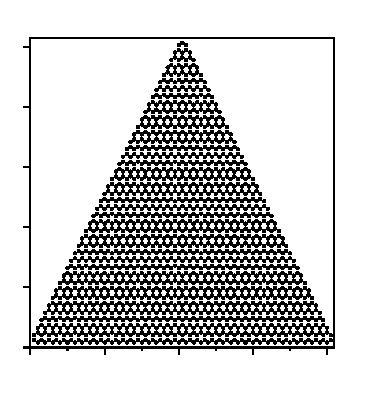
\includegraphics{Coordinates-ZigZag-40}}%
    \gplfronttext
  \end{picture}%
\endgroup

        \captionsetup{width=0.4\textwidth, skip=10pt}
        \caption{A test system --- graphene nanotriangle with zigzag edges of $40\cdot a \approx 10$ nm in width.}
        \label{fig:coordinates-ZigZag-40}
    \end{wrapfigure}
    We start with a toy system --- a small graphene nanotriangle. Picture \ref{fig:coordinates-ZigZag-40} shows the system. It is a flake of $1761$ atomic sites with hexagonal lattice type and graphene lattice constant $a \approx 0.246$ nm. Although the system is about twice as small in width as the triangles discussed in \cite{plasmonic2015}, it is big enough for testing purposes. Our implementation of eq. \eqref{eq:appl:result_w} differs significantly from the one used in \cite{plasmonic2015}. It is thus interesting to check whether both implementations produce the same physical results.

    \texttt{TIPSI} \texttt{Fortran}--\texttt{Python} package \cite{tipsi} suits the task of constructing a tight-binding Hamiltonian rather well. The \hyperref[code]{\texttt{bin/generate\_system.py}} script illustrates how it is done. Graphene lattice constant of $0.246$ nm and the nearest-neighbour hopping value of $2.8$ eV are used.

    \begin{figure}[h]
    \vspace{-0.3cm}
    \begin{minipage}{\textwidth}
        % GNUPLOT: LaTeX picture with Postscript
\begingroup
  \makeatletter
  \providecommand\color[2][]{%
    \GenericError{(gnuplot) \space\space\space\@spaces}{%
      Package color not loaded in conjunction with
      terminal option `colourtext'%
    }{See the gnuplot documentation for explanation.%
    }{Either use 'blacktext' in gnuplot or load the package
      color.sty in LaTeX.}%
    \renewcommand\color[2][]{}%
  }%
  \providecommand\includegraphics[2][]{%
    \GenericError{(gnuplot) \space\space\space\@spaces}{%
      Package graphicx or graphics not loaded%
    }{See the gnuplot documentation for explanation.%
    }{The gnuplot epslatex terminal needs graphicx.sty or graphics.sty.}%
    \renewcommand\includegraphics[2][]{}%
  }%
  \providecommand\rotatebox[2]{#2}%
  \@ifundefined{ifGPcolor}{%
    \newif\ifGPcolor
    \GPcolortrue
  }{}%
  \@ifundefined{ifGPblacktext}{%
    \newif\ifGPblacktext
    \GPblacktexttrue
  }{}%
  % define a \g@addto@macro without @ in the name:
  \let\gplgaddtomacro\g@addto@macro
  % define empty templates for all commands taking text:
  \gdef\gplbacktext{}%
  \gdef\gplfronttext{}%
  \makeatother
  \ifGPblacktext
    % no textcolor at all
    \def\colorrgb#1{}%
    \def\colorgray#1{}%
  \else
    % gray or color?
    \ifGPcolor
      \def\colorrgb#1{\color[rgb]{#1}}%
      \def\colorgray#1{\color[gray]{#1}}%
      \expandafter\def\csname LTw\endcsname{\color{white}}%
      \expandafter\def\csname LTb\endcsname{\color{black}}%
      \expandafter\def\csname LTa\endcsname{\color{black}}%
      \expandafter\def\csname LT0\endcsname{\color[rgb]{1,0,0}}%
      \expandafter\def\csname LT1\endcsname{\color[rgb]{0,1,0}}%
      \expandafter\def\csname LT2\endcsname{\color[rgb]{0,0,1}}%
      \expandafter\def\csname LT3\endcsname{\color[rgb]{1,0,1}}%
      \expandafter\def\csname LT4\endcsname{\color[rgb]{0,1,1}}%
      \expandafter\def\csname LT5\endcsname{\color[rgb]{1,1,0}}%
      \expandafter\def\csname LT6\endcsname{\color[rgb]{0,0,0}}%
      \expandafter\def\csname LT7\endcsname{\color[rgb]{1,0.3,0}}%
      \expandafter\def\csname LT8\endcsname{\color[rgb]{0.5,0.5,0.5}}%
    \else
      % gray
      \def\colorrgb#1{\color{black}}%
      \def\colorgray#1{\color[gray]{#1}}%
      \expandafter\def\csname LTw\endcsname{\color{white}}%
      \expandafter\def\csname LTb\endcsname{\color{black}}%
      \expandafter\def\csname LTa\endcsname{\color{black}}%
      \expandafter\def\csname LT0\endcsname{\color{black}}%
      \expandafter\def\csname LT1\endcsname{\color{black}}%
      \expandafter\def\csname LT2\endcsname{\color{black}}%
      \expandafter\def\csname LT3\endcsname{\color{black}}%
      \expandafter\def\csname LT4\endcsname{\color{black}}%
      \expandafter\def\csname LT5\endcsname{\color{black}}%
      \expandafter\def\csname LT6\endcsname{\color{black}}%
      \expandafter\def\csname LT7\endcsname{\color{black}}%
      \expandafter\def\csname LT8\endcsname{\color{black}}%
    \fi
  \fi
  \setlength{\unitlength}{0.0500bp}%
  \begin{picture}(9636.00,3968.00)%
    \gplgaddtomacro\gplbacktext{%
      \csname LTb\endcsname%
      \put(550,659){\makebox(0,0)[r]{\strut{} 0}}%
      \csname LTb\endcsname%
      \put(550,1276){\makebox(0,0)[r]{\strut{} 1}}%
      \csname LTb\endcsname%
      \put(550,1894){\makebox(0,0)[r]{\strut{} 2}}%
      \csname LTb\endcsname%
      \put(550,2512){\makebox(0,0)[r]{\strut{} 3}}%
      \csname LTb\endcsname%
      \put(550,3129){\makebox(0,0)[r]{\strut{} 4}}%
      \csname LTb\endcsname%
      \put(550,3747){\makebox(0,0)[r]{\strut{} 5}}%
      \csname LTb\endcsname%
      \put(682,440){\makebox(0,0){\strut{} 0.1}}%
      \csname LTb\endcsname%
      \put(1904,440){\makebox(0,0){\strut{} 0.2}}%
      \csname LTb\endcsname%
      \put(3127,440){\makebox(0,0){\strut{} 0.3}}%
      \csname LTb\endcsname%
      \put(4349,440){\makebox(0,0){\strut{} 0.4}}%
      \csname LTb\endcsname%
      \put(5572,440){\makebox(0,0){\strut{} 0.5}}%
      \csname LTb\endcsname%
      \put(6794,440){\makebox(0,0){\strut{} 0.6}}%
      \csname LTb\endcsname%
      \put(8017,440){\makebox(0,0){\strut{} 0.7}}%
      \csname LTb\endcsname%
      \put(9239,440){\makebox(0,0){\strut{} 0.8}}%
      \put(176,2203){\rotatebox{-270}{\makebox(0,0){\strut{}\small{$-\operatorname{Im}[\epsilon_{n(\omega)}^{-1}(\omega)]$}}}}%
      \put(4960,110){\makebox(0,0){\strut{}\small{$\hbar\omega$, eV}}}%
    }%
    \gplgaddtomacro\gplfronttext{%
    }%
    \gplbacktext
    \put(0,0){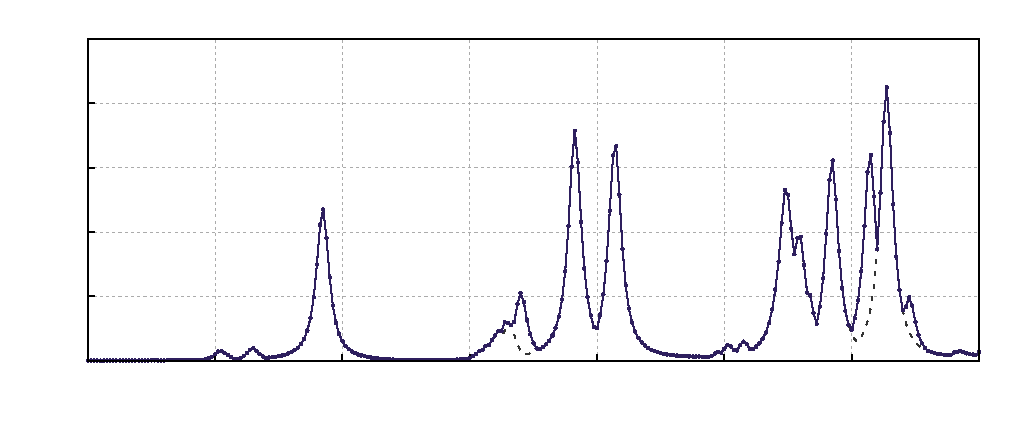
\includegraphics{Spectrum-ZigZag-40}}%
    \gplfronttext
  \end{picture}%
\endgroup

        \captionsetup{skip=5pt}
        \captionof{figure}{Low-energy loss spectrum for a zigzag-edged graphene nanotriangle shown on fig. \ref{fig:coordinates-ZigZag-40}. Solid line shows ``the first maximum'' (i.e. \ $-\operatorname{Im}[\epsilon^{-1}_{n_1(\omega)}(\omega)]$) and dashed lines --- ``the second maximum'' (i.e. \ $-\operatorname{Im}[\epsilon^{-1}_{n_2(\omega)}(\omega)]$).}
        \label{fig:spectrum-ZigZag-40}
    \end{minipage}
    \begin{minipage}{\textwidth}
        \vspace{-1.0cm}
        % GNUPLOT: LaTeX picture with Postscript
\begingroup
  \makeatletter
  \providecommand\color[2][]{%
    \GenericError{(gnuplot) \space\space\space\@spaces}{%
      Package color not loaded in conjunction with
      terminal option `colourtext'%
    }{See the gnuplot documentation for explanation.%
    }{Either use 'blacktext' in gnuplot or load the package
      color.sty in LaTeX.}%
    \renewcommand\color[2][]{}%
  }%
  \providecommand\includegraphics[2][]{%
    \GenericError{(gnuplot) \space\space\space\@spaces}{%
      Package graphicx or graphics not loaded%
    }{See the gnuplot documentation for explanation.%
    }{The gnuplot epslatex terminal needs graphicx.sty or graphics.sty.}%
    \renewcommand\includegraphics[2][]{}%
  }%
  \providecommand\rotatebox[2]{#2}%
  \@ifundefined{ifGPcolor}{%
    \newif\ifGPcolor
    \GPcolortrue
  }{}%
  \@ifundefined{ifGPblacktext}{%
    \newif\ifGPblacktext
    \GPblacktexttrue
  }{}%
  % define a \g@addto@macro without @ in the name:
  \let\gplgaddtomacro\g@addto@macro
  % define empty templates for all commands taking text:
  \gdef\gplbacktext{}%
  \gdef\gplfronttext{}%
  \makeatother
  \ifGPblacktext
    % no textcolor at all
    \def\colorrgb#1{}%
    \def\colorgray#1{}%
  \else
    % gray or color?
    \ifGPcolor
      \def\colorrgb#1{\color[rgb]{#1}}%
      \def\colorgray#1{\color[gray]{#1}}%
      \expandafter\def\csname LTw\endcsname{\color{white}}%
      \expandafter\def\csname LTb\endcsname{\color{black}}%
      \expandafter\def\csname LTa\endcsname{\color{black}}%
      \expandafter\def\csname LT0\endcsname{\color[rgb]{1,0,0}}%
      \expandafter\def\csname LT1\endcsname{\color[rgb]{0,1,0}}%
      \expandafter\def\csname LT2\endcsname{\color[rgb]{0,0,1}}%
      \expandafter\def\csname LT3\endcsname{\color[rgb]{1,0,1}}%
      \expandafter\def\csname LT4\endcsname{\color[rgb]{0,1,1}}%
      \expandafter\def\csname LT5\endcsname{\color[rgb]{1,1,0}}%
      \expandafter\def\csname LT6\endcsname{\color[rgb]{0,0,0}}%
      \expandafter\def\csname LT7\endcsname{\color[rgb]{1,0.3,0}}%
      \expandafter\def\csname LT8\endcsname{\color[rgb]{0.5,0.5,0.5}}%
    \else
      % gray
      \def\colorrgb#1{\color{black}}%
      \def\colorgray#1{\color[gray]{#1}}%
      \expandafter\def\csname LTw\endcsname{\color{white}}%
      \expandafter\def\csname LTb\endcsname{\color{black}}%
      \expandafter\def\csname LTa\endcsname{\color{black}}%
      \expandafter\def\csname LT0\endcsname{\color{black}}%
      \expandafter\def\csname LT1\endcsname{\color{black}}%
      \expandafter\def\csname LT2\endcsname{\color{black}}%
      \expandafter\def\csname LT3\endcsname{\color{black}}%
      \expandafter\def\csname LT4\endcsname{\color{black}}%
      \expandafter\def\csname LT5\endcsname{\color{black}}%
      \expandafter\def\csname LT6\endcsname{\color{black}}%
      \expandafter\def\csname LT7\endcsname{\color{black}}%
      \expandafter\def\csname LT8\endcsname{\color{black}}%
    \fi
  \fi
  \setlength{\unitlength}{0.0500bp}%
  \begin{picture}(10204.00,3968.00)%
    \gplgaddtomacro\gplbacktext{%
    }%
    \gplgaddtomacro\gplfronttext{%
      \csname LTb\endcsname%
      \put(1530,182){\makebox(0,0){\strut{}$\hbar\omega = 0.525$ eV}}%
    }%
    \gplgaddtomacro\gplbacktext{%
    }%
    \gplgaddtomacro\gplfronttext{%
      \csname LTb\endcsname%
      \put(4591,182){\makebox(0,0){\strut{}$\hbar\omega = 0.28$ eV}}%
    }%
    \gplgaddtomacro\gplbacktext{%
    }%
    \gplgaddtomacro\gplfronttext{%
      \csname LTb\endcsname%
      \put(7653,182){\makebox(0,0){\strut{}$\hbar\omega = 0.6875$ eV}}%
      \put(9338,468){\makebox(0,0)[l]{\strut{}\small{-0.06}}}%
      \put(9338,1818){\makebox(0,0)[l]{\strut{}\small{0}}}%
      \put(9338,3168){\makebox(0,0)[l]{\strut{}\small{0.06}}}%
    }%
    \gplbacktext
    \put(0,0){\includegraphics{{{Eigenstates-ZigZag-40}}}}%
    \gplfronttext
  \end{picture}%
\endgroup

        \captionsetup{skip=0pt}
        \captionof{figure}{Some of the plasmon eigenmodes. These eigenmodes were also found by \cite{plasmonic2015}.}
        \label{fig:eigenmodes-ZigZag-40}
    \end{minipage}
    \end{figure}

    We then carry out the diagonalisation of the Hamiltonian using the \hyperref[code]{\texttt{solve\_system}} utility program. Internally a multi-threaded implementation of \texttt{LAPACK} is used which is provided by the \texttt{Intel MKL} \cite{intel-mkl} library.
    
    Next, we use the \hyperref[code]{\texttt{dielectric}} utility to calculate the dielectric function $\hat\varepsilon(\omega)$ for frequencies corresponding to $\hbar\omega \in [0.1,0.8]$ eV. Energy range matches the one used in \cite{plasmonic2015} to allow for comparison of the resulting loss spectra. For the very same reason we also use the same values for the thermodynamic variables: chemical potential $\mu = 0.4$ eV, temperature $T = 300$ K, and ``inverse relaxation time'' $\eta = 6$ meV$\!/\hbar$. Having almost $300$ of $1761\times1761$ matrices is not really representative so we turn to the $\mathbf{r}$--approach to obtain some visualisable results. The loss spectrum, i.e. the \ $-\operatorname{Im}[\hat\varepsilon^{-1}_{n_{\{1, 2\}}(\omega)}(\omega)]$ vs. $\omega$ plot is shown on fig. \ref{fig:spectrum-ZigZag-40}. Solid lines show the ``first maximum'' while dashed lines --- the second. They coincide almost everywhere which is in correspondence with results in \cite{plasmonic2015}. The approximately equal ``frequency'' of the peaks is also reassuring. The first two (due to degeneracy) plasmon eigenmodes even appear at close frequencies: $0.285$ eV (our system) and $0.275$ eV (\!\!\cite{plasmonic2015}); which is amazing taking into account the fact that these systems significantly differ in size.

    \begin{figure}[h] 
    \center
    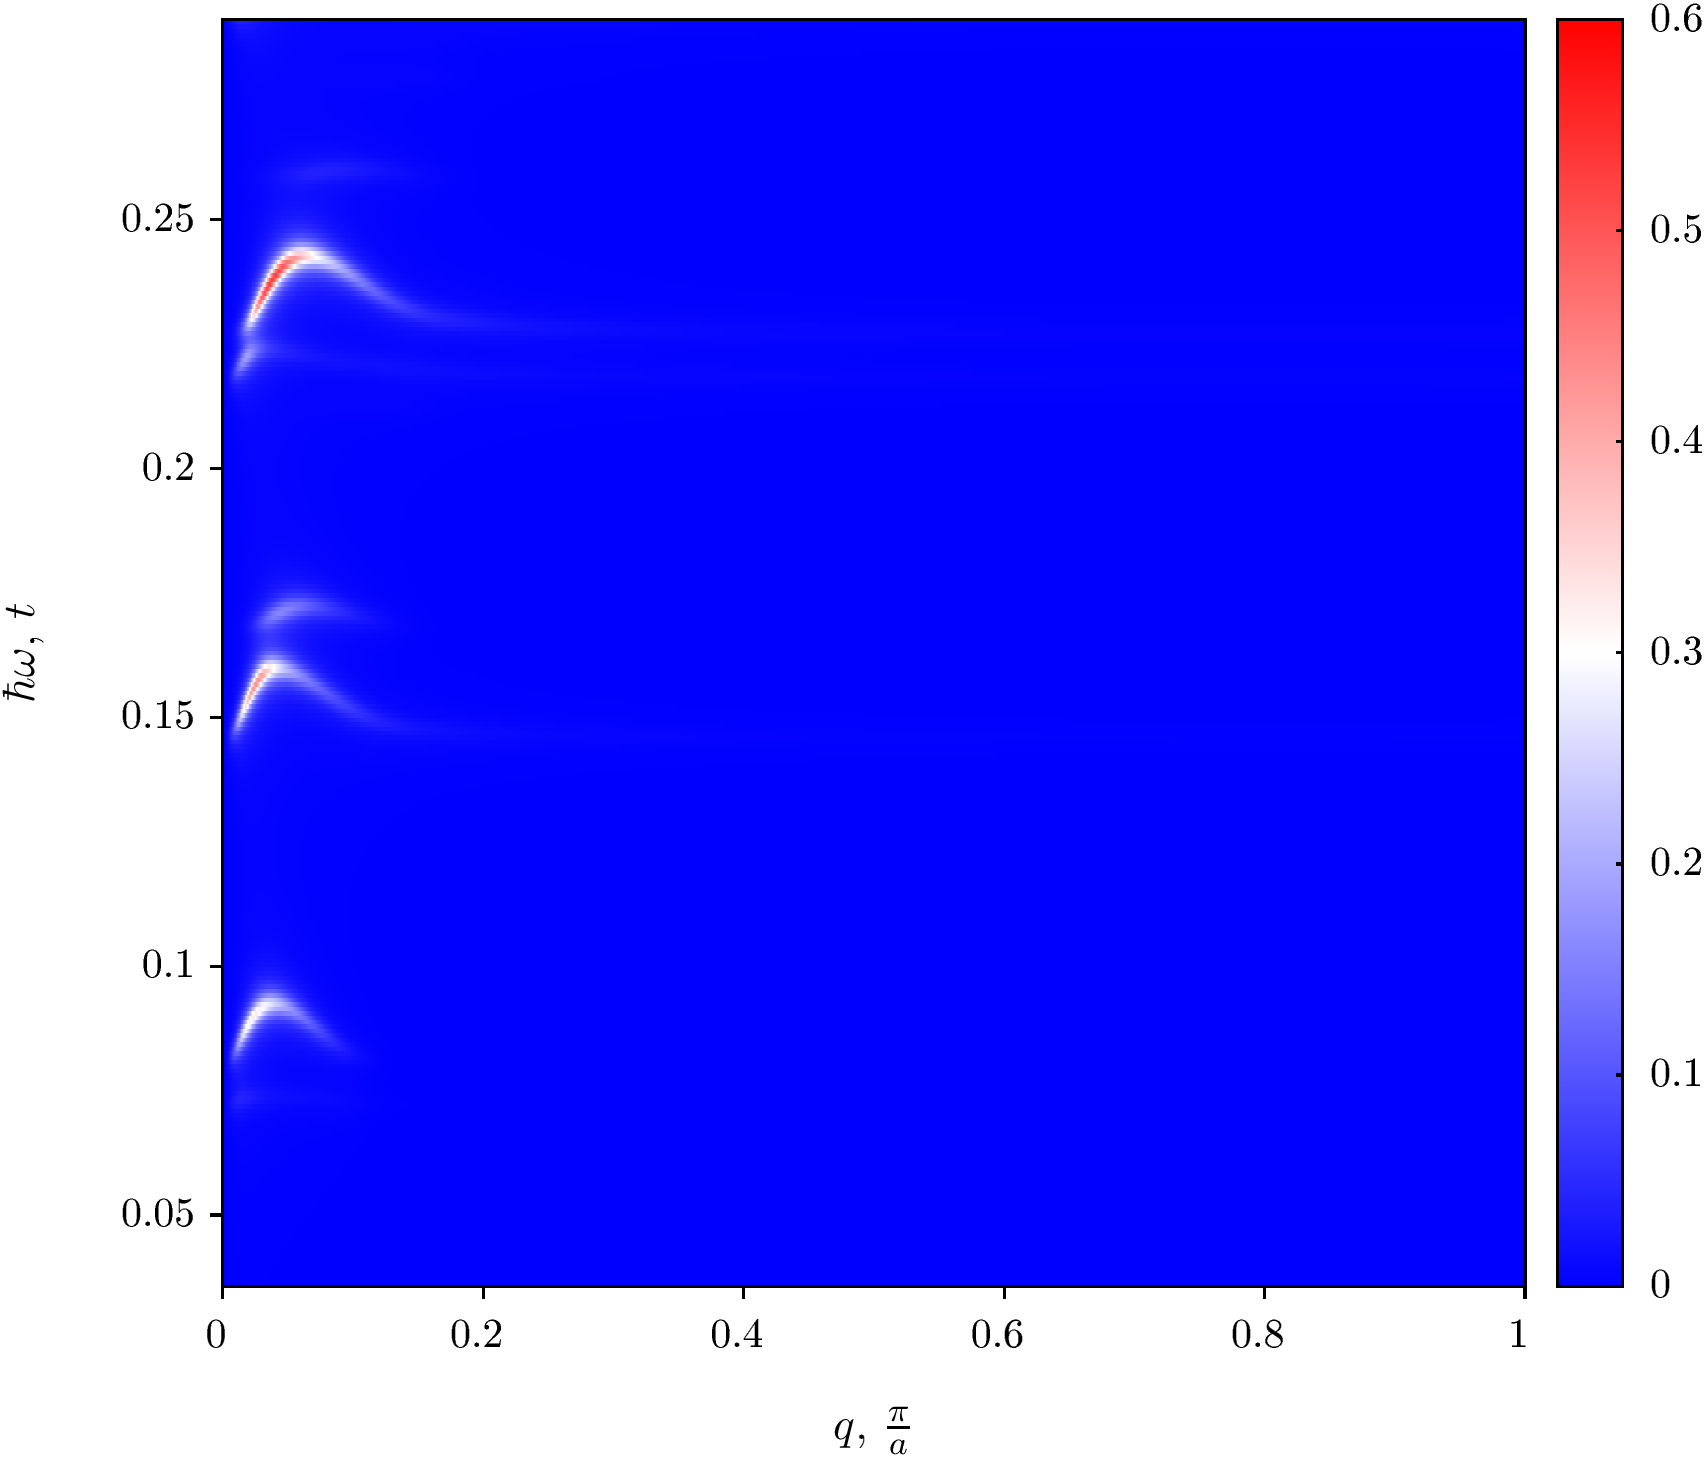
\includegraphics[width=\textwidth]{Spectrum-ZigZag-40-Q-Omega.png}
    \caption{Dispersion relation \ $-\operatorname{Im}[1 / \langle\mathbf{q}| \hat\varepsilon(\omega) |\mathbf{q}\rangle]$ for a zigzag-edged graphene nanotriangle from fig. \ref{fig:coordinates-ZigZag-40}. Momentum $\mathbf{q}$ is in the $x$ direction.}
    \label{fig:spectrum-ZigZag-40-Q-Omega}
    \end{figure}

    We also show a couple of plasmon eigenmodes obtained in the $\mathbf{r}$--approach on fig. \ref{fig:eigenmodes-ZigZag-40}. They also correspond to modes found in \cite{plasmonic2015} which is a good sign meaning we have chosen a big enough system that the boundary effects are not too important.

    We will not discuss the results much further because it has been done extensively in \cite{plasmonic2015}. We do want to show the results of the $\mathbf{q}$--approach, though. The obtained dispersion relation ($-\operatorname{Im}[1 / \langle\mathbf{q}| \hat\varepsilon(\omega) |\mathbf{q}\rangle]$ as a function of $\mathbf{q}$ and $\omega$) is shown on fig. \ref{fig:spectrum-ZigZag-40-Q-Omega}. Although we only see a very narrow range of energies, the picture is still quite interesting. Three ``waves'' appearing at small momenta actually correspond, roughly, to peaks found in the $\mathbf{r}$--approach. This might mean that the $\mathbf{r}$--approach results do hold some physical relevance, contrary to what it might seem at first. An in-depth study of this topic is, however, necessary to make a definitive conclusion.


\subsection{Third iteration Sierpinski carpet}
    \begin{figure}[h]
    \vspace{-0.5cm}
    % GNUPLOT: LaTeX picture with Postscript
\begingroup
  \makeatletter
  \providecommand\color[2][]{%
    \GenericError{(gnuplot) \space\space\space\@spaces}{%
      Package color not loaded in conjunction with
      terminal option `colourtext'%
    }{See the gnuplot documentation for explanation.%
    }{Either use 'blacktext' in gnuplot or load the package
      color.sty in LaTeX.}%
    \renewcommand\color[2][]{}%
  }%
  \providecommand\includegraphics[2][]{%
    \GenericError{(gnuplot) \space\space\space\@spaces}{%
      Package graphicx or graphics not loaded%
    }{See the gnuplot documentation for explanation.%
    }{The gnuplot epslatex terminal needs graphicx.sty or graphics.sty.}%
    \renewcommand\includegraphics[2][]{}%
  }%
  \providecommand\rotatebox[2]{#2}%
  \@ifundefined{ifGPcolor}{%
    \newif\ifGPcolor
    \GPcolortrue
  }{}%
  \@ifundefined{ifGPblacktext}{%
    \newif\ifGPblacktext
    \GPblacktexttrue
  }{}%
  % define a \g@addto@macro without @ in the name:
  \let\gplgaddtomacro\g@addto@macro
  % define empty templates for all commands taking text:
  \gdef\gplbacktext{}%
  \gdef\gplfronttext{}%
  \makeatother
  \ifGPblacktext
    % no textcolor at all
    \def\colorrgb#1{}%
    \def\colorgray#1{}%
  \else
    % gray or color?
    \ifGPcolor
      \def\colorrgb#1{\color[rgb]{#1}}%
      \def\colorgray#1{\color[gray]{#1}}%
      \expandafter\def\csname LTw\endcsname{\color{white}}%
      \expandafter\def\csname LTb\endcsname{\color{black}}%
      \expandafter\def\csname LTa\endcsname{\color{black}}%
      \expandafter\def\csname LT0\endcsname{\color[rgb]{1,0,0}}%
      \expandafter\def\csname LT1\endcsname{\color[rgb]{0,1,0}}%
      \expandafter\def\csname LT2\endcsname{\color[rgb]{0,0,1}}%
      \expandafter\def\csname LT3\endcsname{\color[rgb]{1,0,1}}%
      \expandafter\def\csname LT4\endcsname{\color[rgb]{0,1,1}}%
      \expandafter\def\csname LT5\endcsname{\color[rgb]{1,1,0}}%
      \expandafter\def\csname LT6\endcsname{\color[rgb]{0,0,0}}%
      \expandafter\def\csname LT7\endcsname{\color[rgb]{1,0.3,0}}%
      \expandafter\def\csname LT8\endcsname{\color[rgb]{0.5,0.5,0.5}}%
    \else
      % gray
      \def\colorrgb#1{\color{black}}%
      \def\colorgray#1{\color[gray]{#1}}%
      \expandafter\def\csname LTw\endcsname{\color{white}}%
      \expandafter\def\csname LTb\endcsname{\color{black}}%
      \expandafter\def\csname LTa\endcsname{\color{black}}%
      \expandafter\def\csname LT0\endcsname{\color{black}}%
      \expandafter\def\csname LT1\endcsname{\color{black}}%
      \expandafter\def\csname LT2\endcsname{\color{black}}%
      \expandafter\def\csname LT3\endcsname{\color{black}}%
      \expandafter\def\csname LT4\endcsname{\color{black}}%
      \expandafter\def\csname LT5\endcsname{\color{black}}%
      \expandafter\def\csname LT6\endcsname{\color{black}}%
      \expandafter\def\csname LT7\endcsname{\color{black}}%
      \expandafter\def\csname LT8\endcsname{\color{black}}%
    \fi
  \fi
  \setlength{\unitlength}{0.0500bp}%
  \begin{picture}(7936.00,5102.00)%
    \gplgaddtomacro\gplbacktext{%
      \csname LTb\endcsname%
      \put(682,902){\makebox(0,0)[r]{\strut{} 0}}%
      \put(682,1440){\makebox(0,0)[r]{\strut{} 4}}%
      \put(682,1978){\makebox(0,0)[r]{\strut{} 8}}%
      \put(682,2516){\makebox(0,0)[r]{\strut{} 12}}%
      \put(682,3054){\makebox(0,0)[r]{\strut{} 16}}%
      \put(682,3592){\makebox(0,0)[r]{\strut{} 20}}%
      \put(682,4130){\makebox(0,0)[r]{\strut{} 24}}%
      \put(1008,484){\makebox(0,0){\strut{} 0}}%
      \put(1530,484){\makebox(0,0){\strut{} 4}}%
      \put(2052,484){\makebox(0,0){\strut{} 8}}%
      \put(2575,484){\makebox(0,0){\strut{} 12}}%
      \put(3097,484){\makebox(0,0){\strut{} 16}}%
      \put(3620,484){\makebox(0,0){\strut{} 20}}%
      \put(4142,484){\makebox(0,0){\strut{} 24}}%
      \put(176,2650){\rotatebox{-270}{\makebox(0,0){\strut{}$y$}}}%
      \put(2705,154){\makebox(0,0){\strut{}$x$}}%
      \put(5514,1171){\makebox(0,0)[l]{\strut{}0th iteration (unit cell)}}%
      \put(5514,1440){\makebox(0,0)[l]{\strut{}1st iteration}}%
      \put(5514,2247){\makebox(0,0)[l]{\strut{}2nd iteration}}%
      \put(2706,4779){\makebox(0,0){\strut{}$\approx 6.4$ nm}}%
    }%
    \gplgaddtomacro\gplfronttext{%
    }%
    \gplbacktext
    \put(0,0){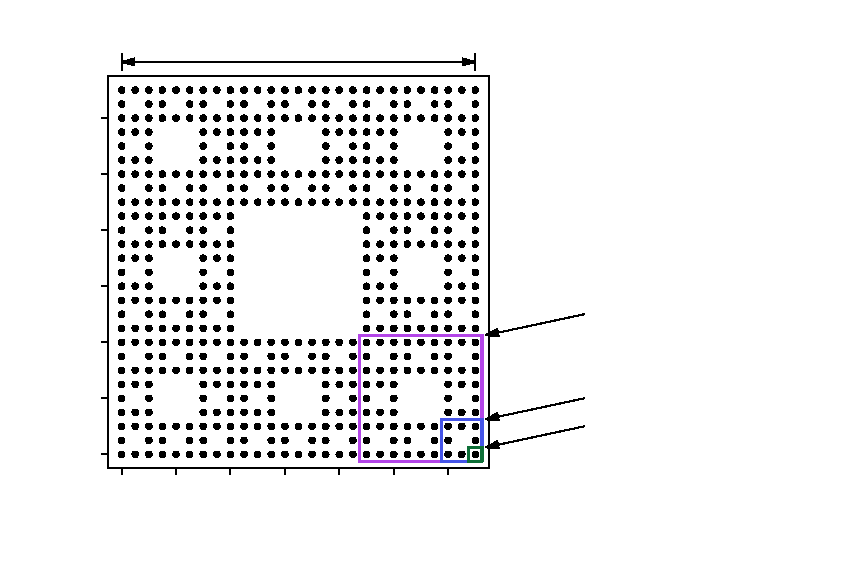
\includegraphics{Coordinates-3rd-SC}}%
    \gplfronttext
  \end{picture}%
\endgroup

    \caption{Third iteration Sierpinski carpet. $x$ and $y$ coordinates are given in terms of lattice constant. Width of the sample is $3^3 = 27$ unit cells. In this case we chose the lattice constant of graphene $a \approx 0.246$ nm, which results in the total width of about six and a half nanometers.}
    \label{fig:coordinates-3rd-SC}
    \end{figure}
    Next, we turn to a somewhat smaller, though a more on-topic, system --- third iteration Siepinski carpet. The sample is shown in fig. \ref{fig:coordinates-3rd-SC}. We again use graphene lattice constant, this due to the need to choose some value\footnote{%
    The method we use here is itself quite generic and can be applied to essentially any lattice constant. It is, however impossible to keep $a$ as a variable due to its appearance in the Coulomb interaction potential. Consider eq. \eqref{eq:appl:result_w}:
    \begin{equation*}
        \langle a | \hat\varepsilon(\omega) | b \rangle
            = \!\!\!\!\!\!\!\!\!\!\!\!\!\!\! \overbrace{\langle a | b \rangle}^\text{\footnotesize independent of $a$} \!\!\!\!\!\!\!\!\!\!\!\!\!\! - \underbrace{\sum_{c} \langle a | \hat V_\text{Coulomb} | c \rangle \langle c | \hat\chi(\omega) | b \rangle}_\text{\footnotesize $\propto 1/a$} \; ,
    \end{equation*}
    so even though we could make the second term on the right-hand side a function of $a$ it is impossible to do so with the right-hand side as a whole. Hence, in general, we can not express $\hat\varepsilon(\omega)$ as a function of $a$. And because there are no experimental papers yet measuring loss function for Sierpinski carpets, it does not really matter which particular value of $a$ we choose. One could claim, however, that the availability of plasmons may depend on $a$ and hence our results are valid for one value of $a$ only. The topic of finding out whether this claim is true or not is better suited for another study.},
    and having graphene-like system lets us compare the results to the ones from sec. \ref{sec:nanotriangles}. All other configuration parameters stay the same, too.
     
    After having obtained eigenenergies of the system in the exact same manner as was explained in sec. \ref{sec:nanotriangles}, we notice that possible energies fall within the $(-9.5\text{ eV}, 9.5\text{ eV})$ range. Hence, $E_i - E_j < 19$ eV for any $i$ and $j$. As we see from eq. \eqref{eq:appl:computing_chi}, $G_{i,j}$ has $(E_i - E_j - \hbar(\omega + i\eta))$ in the denominator, thus for $\omega$'s greater than $\approx20$ eV$/\hbar$ the loss function will asymptotically approach zero --- no need to search for plasmons there. To verify this claim, we calculate $\hat\varepsilon(\omega)$ for frequencies up to $\approx\! 22$ eV.

    \begin{figure}[h]
    \begin{minipage}{.5\textwidth}
        \vspace{-0.5cm}
        % GNUPLOT: LaTeX picture with Postscript
\begingroup
  \makeatletter
  \providecommand\color[2][]{%
    \GenericError{(gnuplot) \space\space\space\@spaces}{%
      Package color not loaded in conjunction with
      terminal option `colourtext'%
    }{See the gnuplot documentation for explanation.%
    }{Either use 'blacktext' in gnuplot or load the package
      color.sty in LaTeX.}%
    \renewcommand\color[2][]{}%
  }%
  \providecommand\includegraphics[2][]{%
    \GenericError{(gnuplot) \space\space\space\@spaces}{%
      Package graphicx or graphics not loaded%
    }{See the gnuplot documentation for explanation.%
    }{The gnuplot epslatex terminal needs graphicx.sty or graphics.sty.}%
    \renewcommand\includegraphics[2][]{}%
  }%
  \providecommand\rotatebox[2]{#2}%
  \@ifundefined{ifGPcolor}{%
    \newif\ifGPcolor
    \GPcolortrue
  }{}%
  \@ifundefined{ifGPblacktext}{%
    \newif\ifGPblacktext
    \GPblacktexttrue
  }{}%
  % define a \g@addto@macro without @ in the name:
  \let\gplgaddtomacro\g@addto@macro
  % define empty templates for all commands taking text:
  \gdef\gplbacktext{}%
  \gdef\gplfronttext{}%
  \makeatother
  \ifGPblacktext
    % no textcolor at all
    \def\colorrgb#1{}%
    \def\colorgray#1{}%
  \else
    % gray or color?
    \ifGPcolor
      \def\colorrgb#1{\color[rgb]{#1}}%
      \def\colorgray#1{\color[gray]{#1}}%
      \expandafter\def\csname LTw\endcsname{\color{white}}%
      \expandafter\def\csname LTb\endcsname{\color{black}}%
      \expandafter\def\csname LTa\endcsname{\color{black}}%
      \expandafter\def\csname LT0\endcsname{\color[rgb]{1,0,0}}%
      \expandafter\def\csname LT1\endcsname{\color[rgb]{0,1,0}}%
      \expandafter\def\csname LT2\endcsname{\color[rgb]{0,0,1}}%
      \expandafter\def\csname LT3\endcsname{\color[rgb]{1,0,1}}%
      \expandafter\def\csname LT4\endcsname{\color[rgb]{0,1,1}}%
      \expandafter\def\csname LT5\endcsname{\color[rgb]{1,1,0}}%
      \expandafter\def\csname LT6\endcsname{\color[rgb]{0,0,0}}%
      \expandafter\def\csname LT7\endcsname{\color[rgb]{1,0.3,0}}%
      \expandafter\def\csname LT8\endcsname{\color[rgb]{0.5,0.5,0.5}}%
    \else
      % gray
      \def\colorrgb#1{\color{black}}%
      \def\colorgray#1{\color[gray]{#1}}%
      \expandafter\def\csname LTw\endcsname{\color{white}}%
      \expandafter\def\csname LTb\endcsname{\color{black}}%
      \expandafter\def\csname LTa\endcsname{\color{black}}%
      \expandafter\def\csname LT0\endcsname{\color{black}}%
      \expandafter\def\csname LT1\endcsname{\color{black}}%
      \expandafter\def\csname LT2\endcsname{\color{black}}%
      \expandafter\def\csname LT3\endcsname{\color{black}}%
      \expandafter\def\csname LT4\endcsname{\color{black}}%
      \expandafter\def\csname LT5\endcsname{\color{black}}%
      \expandafter\def\csname LT6\endcsname{\color{black}}%
      \expandafter\def\csname LT7\endcsname{\color{black}}%
      \expandafter\def\csname LT8\endcsname{\color{black}}%
    \fi
  \fi
  \setlength{\unitlength}{0.0500bp}%
  \begin{picture}(4534.00,2834.00)%
    \gplgaddtomacro\gplbacktext{%
      \csname LTb\endcsname%
      \put(550,594){\makebox(0,0)[r]{\strut{} 0}}%
      \csname LTb\endcsname%
      \put(550,1055){\makebox(0,0)[r]{\strut{}}}%
      \csname LTb\endcsname%
      \put(550,1516){\makebox(0,0)[r]{\strut{}}}%
      \csname LTb\endcsname%
      \put(550,1977){\makebox(0,0)[r]{\strut{}}}%
      \csname LTb\endcsname%
      \put(550,2437){\makebox(0,0)[r]{\strut{}}}%
      \csname LTb\endcsname%
      \put(958,374){\makebox(0,0){\strut{} 7.2}}%
      \csname LTb\endcsname%
      \put(1442,374){\makebox(0,0){\strut{} 7.3}}%
      \csname LTb\endcsname%
      \put(1926,374){\makebox(0,0){\strut{} 7.4}}%
      \csname LTb\endcsname%
      \put(2409,374){\makebox(0,0){\strut{} 7.5}}%
      \csname LTb\endcsname%
      \put(2893,374){\makebox(0,0){\strut{} 7.6}}%
      \csname LTb\endcsname%
      \put(3377,374){\makebox(0,0){\strut{} 7.7}}%
      \csname LTb\endcsname%
      \put(3861,374){\makebox(0,0){\strut{} 7.8}}%
      \put(176,1581){\rotatebox{-270}{\makebox(0,0){\strut{}\small{$-\operatorname{Im}[\epsilon_{n_1(\omega)}^{-1}(\omega)]$}}}}%
      \put(2409,154){\makebox(0,0){\strut{}\small{$\hbar\omega$, $t$}}}%
    }%
    \gplgaddtomacro\gplfronttext{%
      \csname LTb\endcsname%
      \put(3150,2396){\makebox(0,0)[r]{\strut{}\footnotesize{Fit}}}%
      \csname LTb\endcsname%
      \put(3150,2176){\makebox(0,0)[r]{\strut{}\footnotesize{Numerical}}}%
    }%
    \gplbacktext
    \put(0,0){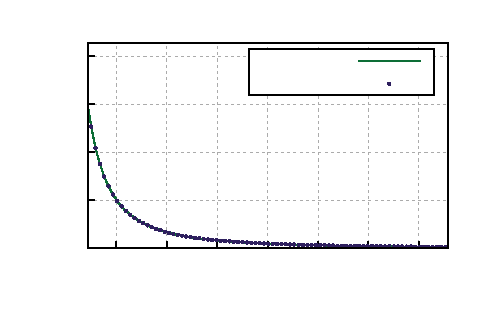
\includegraphics{Spectrum-3rd-SC-Asymptotic}}%
    \gplfronttext
  \end{picture}%
\endgroup

        \captionsetup{width=0.95\linewidth}
        \captionof{figure}{This plot shows asymptotic behavior of \ $-\operatorname{Im}[\hat\varepsilon^{-1}_{n_1(\omega)}(\omega)]$ at high frequencies. Loss function (in arbitrary units) is plotted against electron energy loss (in $t$, hopping value). ``Numerical'' curve is the result of the precise numerical calculation. ``Fit'' is obtained by fitting $a / ((b - \omega)^2 + c^2)$ (i.e. eq. \eqref{eq:exp:asymptotic_approx}) to the results of numerical calculations.} 
        \label{fig:spectrum-3rd-SC-Asymptotic}
    \end{minipage}%
    \begin{minipage}{.5\textwidth}
        \vspace{-0.5cm}
        % GNUPLOT: LaTeX picture with Postscript
\begingroup
  \makeatletter
  \providecommand\color[2][]{%
    \GenericError{(gnuplot) \space\space\space\@spaces}{%
      Package color not loaded in conjunction with
      terminal option `colourtext'%
    }{See the gnuplot documentation for explanation.%
    }{Either use 'blacktext' in gnuplot or load the package
      color.sty in LaTeX.}%
    \renewcommand\color[2][]{}%
  }%
  \providecommand\includegraphics[2][]{%
    \GenericError{(gnuplot) \space\space\space\@spaces}{%
      Package graphicx or graphics not loaded%
    }{See the gnuplot documentation for explanation.%
    }{The gnuplot epslatex terminal needs graphicx.sty or graphics.sty.}%
    \renewcommand\includegraphics[2][]{}%
  }%
  \providecommand\rotatebox[2]{#2}%
  \@ifundefined{ifGPcolor}{%
    \newif\ifGPcolor
    \GPcolortrue
  }{}%
  \@ifundefined{ifGPblacktext}{%
    \newif\ifGPblacktext
    \GPblacktexttrue
  }{}%
  % define a \g@addto@macro without @ in the name:
  \let\gplgaddtomacro\g@addto@macro
  % define empty templates for all commands taking text:
  \gdef\gplbacktext{}%
  \gdef\gplfronttext{}%
  \makeatother
  \ifGPblacktext
    % no textcolor at all
    \def\colorrgb#1{}%
    \def\colorgray#1{}%
  \else
    % gray or color?
    \ifGPcolor
      \def\colorrgb#1{\color[rgb]{#1}}%
      \def\colorgray#1{\color[gray]{#1}}%
      \expandafter\def\csname LTw\endcsname{\color{white}}%
      \expandafter\def\csname LTb\endcsname{\color{black}}%
      \expandafter\def\csname LTa\endcsname{\color{black}}%
      \expandafter\def\csname LT0\endcsname{\color[rgb]{1,0,0}}%
      \expandafter\def\csname LT1\endcsname{\color[rgb]{0,1,0}}%
      \expandafter\def\csname LT2\endcsname{\color[rgb]{0,0,1}}%
      \expandafter\def\csname LT3\endcsname{\color[rgb]{1,0,1}}%
      \expandafter\def\csname LT4\endcsname{\color[rgb]{0,1,1}}%
      \expandafter\def\csname LT5\endcsname{\color[rgb]{1,1,0}}%
      \expandafter\def\csname LT6\endcsname{\color[rgb]{0,0,0}}%
      \expandafter\def\csname LT7\endcsname{\color[rgb]{1,0.3,0}}%
      \expandafter\def\csname LT8\endcsname{\color[rgb]{0.5,0.5,0.5}}%
    \else
      % gray
      \def\colorrgb#1{\color{black}}%
      \def\colorgray#1{\color[gray]{#1}}%
      \expandafter\def\csname LTw\endcsname{\color{white}}%
      \expandafter\def\csname LTb\endcsname{\color{black}}%
      \expandafter\def\csname LTa\endcsname{\color{black}}%
      \expandafter\def\csname LT0\endcsname{\color{black}}%
      \expandafter\def\csname LT1\endcsname{\color{black}}%
      \expandafter\def\csname LT2\endcsname{\color{black}}%
      \expandafter\def\csname LT3\endcsname{\color{black}}%
      \expandafter\def\csname LT4\endcsname{\color{black}}%
      \expandafter\def\csname LT5\endcsname{\color{black}}%
      \expandafter\def\csname LT6\endcsname{\color{black}}%
      \expandafter\def\csname LT7\endcsname{\color{black}}%
      \expandafter\def\csname LT8\endcsname{\color{black}}%
    \fi
  \fi
  \setlength{\unitlength}{0.0500bp}%
  \begin{picture}(4534.00,2834.00)%
    \gplgaddtomacro\gplbacktext{%
      \csname LTb\endcsname%
      \put(550,594){\makebox(0,0)[r]{\strut{}}}%
      \csname LTb\endcsname%
      \put(550,923){\makebox(0,0)[r]{\strut{}}}%
      \csname LTb\endcsname%
      \put(550,1252){\makebox(0,0)[r]{\strut{}$0$}}%
      \csname LTb\endcsname%
      \put(550,1582){\makebox(0,0)[r]{\strut{}}}%
      \csname LTb\endcsname%
      \put(550,1911){\makebox(0,0)[r]{\strut{}}}%
      \csname LTb\endcsname%
      \put(550,2240){\makebox(0,0)[r]{\strut{}}}%
      \csname LTb\endcsname%
      \put(550,2569){\makebox(0,0)[r]{\strut{}}}%
      \csname LTb\endcsname%
      \put(682,374){\makebox(0,0){\strut{}$0.3$}}%
      \csname LTb\endcsname%
      \put(1258,374){\makebox(0,0){\strut{}}}%
      \csname LTb\endcsname%
      \put(1834,374){\makebox(0,0){\strut{}$0.32$}}%
      \csname LTb\endcsname%
      \put(2410,374){\makebox(0,0){\strut{}}}%
      \csname LTb\endcsname%
      \put(2985,374){\makebox(0,0){\strut{}$0.34$}}%
      \csname LTb\endcsname%
      \put(3561,374){\makebox(0,0){\strut{}}}%
      \csname LTb\endcsname%
      \put(4137,374){\makebox(0,0){\strut{}$0.36$}}%
      \put(176,1581){\rotatebox{-270}{\makebox(0,0){\strut{}\small{$\operatorname{Re}[\epsilon_{n_1(\omega)}(\omega)]$}}}}%
      \put(2409,154){\makebox(0,0){\strut{}\small{$\hbar\omega$, eV}}}%
    }%
    \gplgaddtomacro\gplfronttext{%
    }%
    \gplbacktext
    \put(0,0){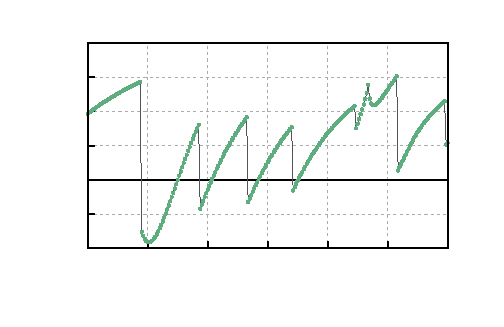
\includegraphics{Spectrum-3rd-SC-Real}}%
    \gplfronttext
  \end{picture}%
\endgroup

        \captionsetup{width=0.95\linewidth}
        \captionof{figure}{Behavior of $\operatorname{Re}[\epsilon_{n(\omega)}(\omega)]$ is shown. A really narrow interval of frequencies is chosen for clarity. \\\hfill\\\hfill \\\hfill \\\hfill \\\hfill}
        \label{fig:spectrum-3rd-SC-real}
    \end{minipage}
    \begin{minipage}{\textwidth}
        % \begin{figure}[h] 
        % \center
        % GNUPLOT: LaTeX picture with Postscript
\begingroup
  \makeatletter
  \providecommand\color[2][]{%
    \GenericError{(gnuplot) \space\space\space\@spaces}{%
      Package color not loaded in conjunction with
      terminal option `colourtext'%
    }{See the gnuplot documentation for explanation.%
    }{Either use 'blacktext' in gnuplot or load the package
      color.sty in LaTeX.}%
    \renewcommand\color[2][]{}%
  }%
  \providecommand\includegraphics[2][]{%
    \GenericError{(gnuplot) \space\space\space\@spaces}{%
      Package graphicx or graphics not loaded%
    }{See the gnuplot documentation for explanation.%
    }{The gnuplot epslatex terminal needs graphicx.sty or graphics.sty.}%
    \renewcommand\includegraphics[2][]{}%
  }%
  \providecommand\rotatebox[2]{#2}%
  \@ifundefined{ifGPcolor}{%
    \newif\ifGPcolor
    \GPcolortrue
  }{}%
  \@ifundefined{ifGPblacktext}{%
    \newif\ifGPblacktext
    \GPblacktexttrue
  }{}%
  % define a \g@addto@macro without @ in the name:
  \let\gplgaddtomacro\g@addto@macro
  % define empty templates for all commands taking text:
  \gdef\gplbacktext{}%
  \gdef\gplfronttext{}%
  \makeatother
  \ifGPblacktext
    % no textcolor at all
    \def\colorrgb#1{}%
    \def\colorgray#1{}%
  \else
    % gray or color?
    \ifGPcolor
      \def\colorrgb#1{\color[rgb]{#1}}%
      \def\colorgray#1{\color[gray]{#1}}%
      \expandafter\def\csname LTw\endcsname{\color{white}}%
      \expandafter\def\csname LTb\endcsname{\color{black}}%
      \expandafter\def\csname LTa\endcsname{\color{black}}%
      \expandafter\def\csname LT0\endcsname{\color[rgb]{1,0,0}}%
      \expandafter\def\csname LT1\endcsname{\color[rgb]{0,1,0}}%
      \expandafter\def\csname LT2\endcsname{\color[rgb]{0,0,1}}%
      \expandafter\def\csname LT3\endcsname{\color[rgb]{1,0,1}}%
      \expandafter\def\csname LT4\endcsname{\color[rgb]{0,1,1}}%
      \expandafter\def\csname LT5\endcsname{\color[rgb]{1,1,0}}%
      \expandafter\def\csname LT6\endcsname{\color[rgb]{0,0,0}}%
      \expandafter\def\csname LT7\endcsname{\color[rgb]{1,0.3,0}}%
      \expandafter\def\csname LT8\endcsname{\color[rgb]{0.5,0.5,0.5}}%
    \else
      % gray
      \def\colorrgb#1{\color{black}}%
      \def\colorgray#1{\color[gray]{#1}}%
      \expandafter\def\csname LTw\endcsname{\color{white}}%
      \expandafter\def\csname LTb\endcsname{\color{black}}%
      \expandafter\def\csname LTa\endcsname{\color{black}}%
      \expandafter\def\csname LT0\endcsname{\color{black}}%
      \expandafter\def\csname LT1\endcsname{\color{black}}%
      \expandafter\def\csname LT2\endcsname{\color{black}}%
      \expandafter\def\csname LT3\endcsname{\color{black}}%
      \expandafter\def\csname LT4\endcsname{\color{black}}%
      \expandafter\def\csname LT5\endcsname{\color{black}}%
      \expandafter\def\csname LT6\endcsname{\color{black}}%
      \expandafter\def\csname LT7\endcsname{\color{black}}%
      \expandafter\def\csname LT8\endcsname{\color{black}}%
    \fi
  \fi
  \setlength{\unitlength}{0.0500bp}%
  \begin{picture}(9636.00,4534.00)%
    \gplgaddtomacro\gplbacktext{%
      \csname LTb\endcsname%
      \put(814,704){\makebox(0,0)[r]{\strut{} 0}}%
      \csname LTb\endcsname%
      \put(814,1595){\makebox(0,0)[r]{\strut{} 100}}%
      \csname LTb\endcsname%
      \put(814,2486){\makebox(0,0)[r]{\strut{} 200}}%
      \csname LTb\endcsname%
      \put(814,3378){\makebox(0,0)[r]{\strut{} 300}}%
      \csname LTb\endcsname%
      \put(814,4269){\makebox(0,0)[r]{\strut{} 400}}%
      \csname LTb\endcsname%
      \put(946,484){\makebox(0,0){\strut{} 0}}%
      \csname LTb\endcsname%
      \put(2077,484){\makebox(0,0){\strut{} 3}}%
      \csname LTb\endcsname%
      \put(3208,484){\makebox(0,0){\strut{} 6}}%
      \csname LTb\endcsname%
      \put(4339,484){\makebox(0,0){\strut{} 9}}%
      \csname LTb\endcsname%
      \put(5469,484){\makebox(0,0){\strut{} 12}}%
      \csname LTb\endcsname%
      \put(6600,484){\makebox(0,0){\strut{} 15}}%
      \csname LTb\endcsname%
      \put(7731,484){\makebox(0,0){\strut{} 18}}%
      \csname LTb\endcsname%
      \put(8862,484){\makebox(0,0){\strut{} 21}}%
      \put(176,2486){\rotatebox{-270}{\makebox(0,0){\strut{}$-\operatorname{Im}[\epsilon_{n_1(\omega)}^{-1}(\omega)]$}}}%
      \put(5092,154){\makebox(0,0){\strut{}$\hbar\omega$, eV}}%
    }%
    \gplgaddtomacro\gplfronttext{%
    }%
    \gplgaddtomacro\gplbacktext{%
    }%
    \gplgaddtomacro\gplfronttext{%
      \csname LTb\endcsname%
      \put(1907,2026){\makebox(0,0)[r]{\strut{}\footnotesize{0}}}%
      \put(1907,2698){\makebox(0,0)[r]{\strut{}\footnotesize{1}}}%
      \put(1907,3370){\makebox(0,0)[r]{\strut{}\footnotesize{2}}}%
      \put(1907,4042){\makebox(0,0)[r]{\strut{}\footnotesize{3}}}%
      \put(2039,1806){\makebox(0,0){\strut{}\footnotesize{0.4}}}%
      \put(3953,1806){\makebox(0,0){\strut{}\footnotesize{0.5}}}%
      \put(5866,1806){\makebox(0,0){\strut{}\footnotesize{0.6}}}%
    }%
    \gplbacktext
    \put(0,0){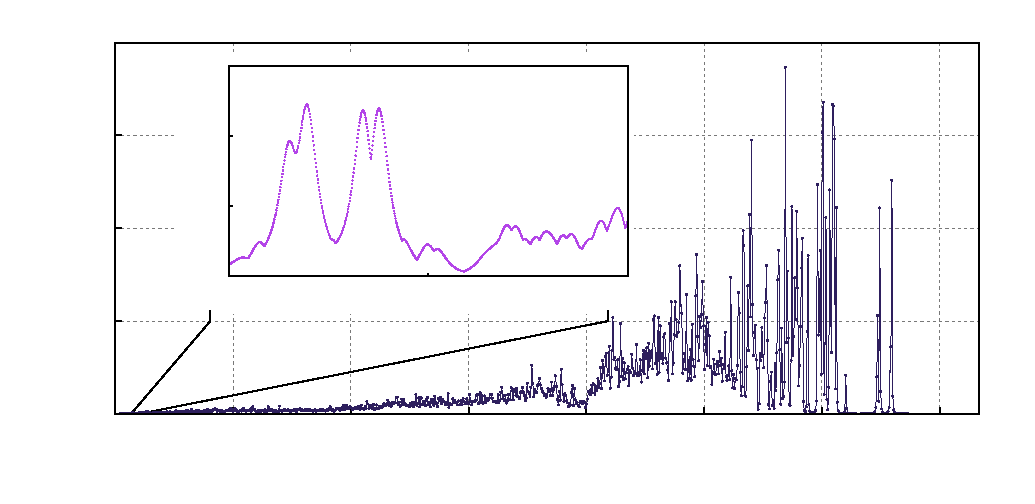
\includegraphics{Spectrum-3rd-SC-Far-Away}}%
    \gplfronttext
  \end{picture}%
\endgroup

        \captionof{figure}{Loss function spectrum for the third iteration Sierpinski carpet.}
        \label{fig:spectrum-3rd-SC-far-away}
        % \end{figure}
    \end{minipage}
    \end{figure}
    
    Let us ignore for a minute the fact that $\hat\epsilon(\omega)$ is a matrix. Using eq. \eqref{eq:appl:result_w} we can approximate it by 
    \begin{equation*}
        \epsilon(\omega) \approx 1 - \frac{A}{B - \omega + i\cdot C} \; ,
    \end{equation*}
    where $A$, $B$, and $C$ are some fitting parameters. This expression is called the \textit{single-pole model} in \cite{andersen2012spatially}. The loss function now becomes\footnote{ %
    \begin{equation*}
        \begin{aligned}
        -\operatorname{Im}[\epsilon(\omega)^{-1}] &= -\operatorname{Im}\left[\left(1 - \frac{A}{B - \omega + i\cdot C}\right)^{-1}\right]
        = -\operatorname{Im}\left[\frac{B - \omega + i\cdot C}{B - A - \omega + i\cdot C}\right] \\
        &= -\operatorname{Im}\left[\frac{(B - \omega + i\cdot C)(B - A - \omega - i\cdot C)}{(B - A - \omega)^2 + C^2}\right]
        = -\frac{-C(B - \omega) + C(B - A - \omega)}{(B - A - \omega)^2 + C^2} \\
        &= \frac{CA}{(B - A - \omega)^2 + C^2} \; .
        \end{aligned}
    \end{equation*}
    } % end footnote
    \begin{equation} \label{eq:exp:asymptotic_approx}
        -\operatorname{Im}\left[\frac{1}{\epsilon(\omega)}\right] \approx \frac{a}{(b - \omega)^2 + c^2} \;,\text{ where }a=AC ,\;\; b = B-A ,\;\; c = C\;.
    \end{equation}
    Fig. \ref{fig:spectrum-3rd-SC-Asymptotic} shows the fit of this expression to the calculated \ $-\operatorname{Im}[\hat\varepsilon^{-1}_{n_1(\omega)}(\omega)]$. As we see, this model describes the loss function very well for energies higher than $\underset{i,j}{\operatorname{max}}|E_i - E_j|$. And although we only fitted the loss function obtained in the $\mathbf{r}$--approach, we know that the loss function in the $\mathbf{q}$--approach decays as well. $n_1(\omega)$ is the index of the eigenvalue whose inverse has the highest imaginary part. We thus know that imaginary parts of inverses of all other eigenvalues decay at least as fast. And thus a linear combination of them with coefficients smaller than one does so as well.

    \begin{figure}[h] 
    \center
    % GNUPLOT: LaTeX picture with Postscript
\begingroup
  \makeatletter
  \providecommand\color[2][]{%
    \GenericError{(gnuplot) \space\space\space\@spaces}{%
      Package color not loaded in conjunction with
      terminal option `colourtext'%
    }{See the gnuplot documentation for explanation.%
    }{Either use 'blacktext' in gnuplot or load the package
      color.sty in LaTeX.}%
    \renewcommand\color[2][]{}%
  }%
  \providecommand\includegraphics[2][]{%
    \GenericError{(gnuplot) \space\space\space\@spaces}{%
      Package graphicx or graphics not loaded%
    }{See the gnuplot documentation for explanation.%
    }{The gnuplot epslatex terminal needs graphicx.sty or graphics.sty.}%
    \renewcommand\includegraphics[2][]{}%
  }%
  \providecommand\rotatebox[2]{#2}%
  \@ifundefined{ifGPcolor}{%
    \newif\ifGPcolor
    \GPcolortrue
  }{}%
  \@ifundefined{ifGPblacktext}{%
    \newif\ifGPblacktext
    \GPblacktexttrue
  }{}%
  % define a \g@addto@macro without @ in the name:
  \let\gplgaddtomacro\g@addto@macro
  % define empty templates for all commands taking text:
  \gdef\gplbacktext{}%
  \gdef\gplfronttext{}%
  \makeatother
  \ifGPblacktext
    % no textcolor at all
    \def\colorrgb#1{}%
    \def\colorgray#1{}%
  \else
    % gray or color?
    \ifGPcolor
      \def\colorrgb#1{\color[rgb]{#1}}%
      \def\colorgray#1{\color[gray]{#1}}%
      \expandafter\def\csname LTw\endcsname{\color{white}}%
      \expandafter\def\csname LTb\endcsname{\color{black}}%
      \expandafter\def\csname LTa\endcsname{\color{black}}%
      \expandafter\def\csname LT0\endcsname{\color[rgb]{1,0,0}}%
      \expandafter\def\csname LT1\endcsname{\color[rgb]{0,1,0}}%
      \expandafter\def\csname LT2\endcsname{\color[rgb]{0,0,1}}%
      \expandafter\def\csname LT3\endcsname{\color[rgb]{1,0,1}}%
      \expandafter\def\csname LT4\endcsname{\color[rgb]{0,1,1}}%
      \expandafter\def\csname LT5\endcsname{\color[rgb]{1,1,0}}%
      \expandafter\def\csname LT6\endcsname{\color[rgb]{0,0,0}}%
      \expandafter\def\csname LT7\endcsname{\color[rgb]{1,0.3,0}}%
      \expandafter\def\csname LT8\endcsname{\color[rgb]{0.5,0.5,0.5}}%
    \else
      % gray
      \def\colorrgb#1{\color{black}}%
      \def\colorgray#1{\color[gray]{#1}}%
      \expandafter\def\csname LTw\endcsname{\color{white}}%
      \expandafter\def\csname LTb\endcsname{\color{black}}%
      \expandafter\def\csname LTa\endcsname{\color{black}}%
      \expandafter\def\csname LT0\endcsname{\color{black}}%
      \expandafter\def\csname LT1\endcsname{\color{black}}%
      \expandafter\def\csname LT2\endcsname{\color{black}}%
      \expandafter\def\csname LT3\endcsname{\color{black}}%
      \expandafter\def\csname LT4\endcsname{\color{black}}%
      \expandafter\def\csname LT5\endcsname{\color{black}}%
      \expandafter\def\csname LT6\endcsname{\color{black}}%
      \expandafter\def\csname LT7\endcsname{\color{black}}%
      \expandafter\def\csname LT8\endcsname{\color{black}}%
    \fi
  \fi
  \setlength{\unitlength}{0.0500bp}%
  \begin{picture}(9636.00,5668.00)%
    \gplgaddtomacro\gplbacktext{%
      \csname LTb\endcsname%
      \put(946,704){\makebox(0,0)[r]{\strut{} 0}}%
      \csname LTb\endcsname%
      \put(946,1644){\makebox(0,0)[r]{\strut{} 0.5}}%
      \csname LTb\endcsname%
      \put(946,2584){\makebox(0,0)[r]{\strut{} 1}}%
      \csname LTb\endcsname%
      \put(946,3523){\makebox(0,0)[r]{\strut{} 1.5}}%
      \csname LTb\endcsname%
      \put(946,4463){\makebox(0,0)[r]{\strut{} 2}}%
      \csname LTb\endcsname%
      \put(946,5403){\makebox(0,0)[r]{\strut{} 2.5}}%
      \csname LTb\endcsname%
      \put(1078,484){\makebox(0,0){\strut{} 0.4}}%
      \csname LTb\endcsname%
      \put(2438,484){\makebox(0,0){\strut{} 0.45}}%
      \csname LTb\endcsname%
      \put(3798,484){\makebox(0,0){\strut{} 0.5}}%
      \csname LTb\endcsname%
      \put(5159,484){\makebox(0,0){\strut{} 0.55}}%
      \csname LTb\endcsname%
      \put(6519,484){\makebox(0,0){\strut{} 0.6}}%
      \csname LTb\endcsname%
      \put(7879,484){\makebox(0,0){\strut{} 0.65}}%
      \csname LTb\endcsname%
      \put(9239,484){\makebox(0,0){\strut{} 0.7}}%
      \put(176,3053){\rotatebox{-270}{\makebox(0,0){\strut{}$-\operatorname{Im}[\epsilon_{n(\omega)}^{-1}(\omega)]$}}}%
      \put(5158,154){\makebox(0,0){\strut{}$\hbar\omega$, eV}}%
    }%
    \gplgaddtomacro\gplfronttext{%
    }%
    \gplbacktext
    \put(0,0){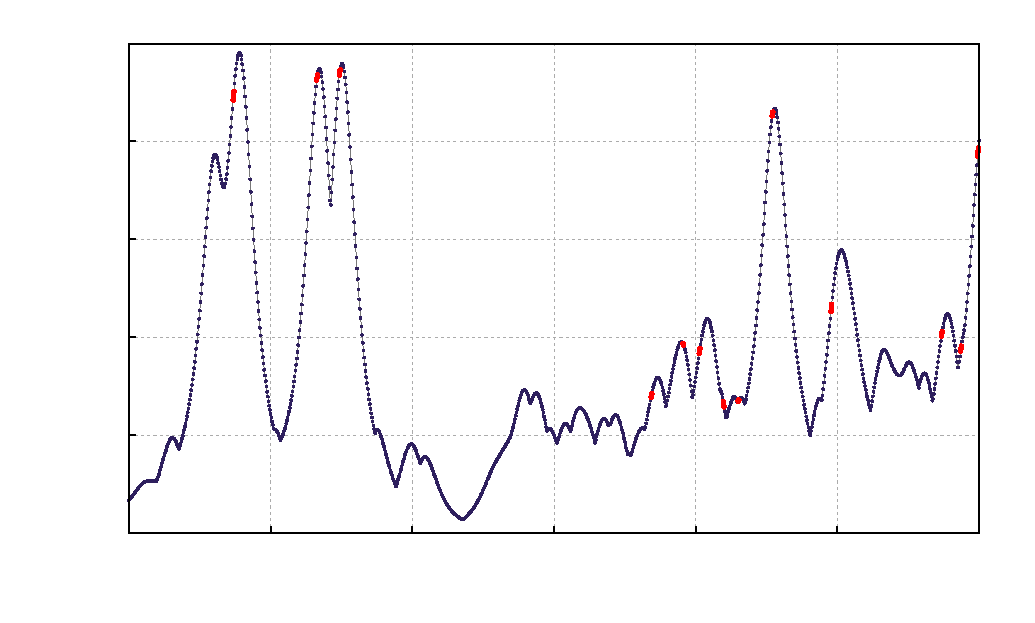
\includegraphics{Spectrum-3rd-SC}}%
    \gplfronttext
  \end{picture}%
\endgroup

    \caption{Loss function spectrum with ``classical'' plasmons marked in red. Each pair of dots indicates a range where the real part of the dielectric function switches sign.}
    \label{fig:spectrum-3rd-SC}
    \end{figure}

    We first consider the loss function as defined in \cite{plasmonic2015}. Loss spectrum for the full range of calculated frequencies is shown on fig. \ref{fig:spectrum-3rd-SC-far-away}. High number of sharp peaks implies that there is a handful of plasmons. On one hand, this means lots of possibilities for experimental applications. On the other hand, we see no similar spectra reported by experimental physicists. It is still unclear whether the results obtained in the $\mathbf{r}$--approach can be realised experimentally.
    %This might mean that the results obtained in the $\mathbf{r}$--approach are unphysical and have no correspondence to experiments.
    
    It is interesting to compare the classical definition of plasmon (i.e. condition \eqref{eq:exp:plasmon_def}) to the condition that loss function has a local maximum. Fig. \ref{fig:spectrum-3rd-SC-real} shows the behavior of the real part of the dielectric function $\epsilon_{n_1(\omega)}(\omega)$. And although the plot shows a very narrow range of energies, $\operatorname{Re} [\epsilon_{n_1(\omega)}(\omega)]$ exhibits similar behavior in general. We only identify the actual roots (not points of discontinuity) with plasmon frequencies.
    
    Fig. \ref{fig:spectrum-3rd-SC} shows the infrared part\footnote{%
        Because low-energy plasmons are easier to excite experimentally. 
    } of the loss spectrum (fig. \ref{fig:spectrum-3rd-SC-far-away}) with red dashes marking the intervals where the real part of the dielectric function switches sign from \ $-1$ to $+1$. We see that ``classical'' plasmon frequencies are indeed located near maxima of the loss function. As noted by \cite{andersen2012spatially}, it is unimportant that the peaks do not coincide with roots of $\operatorname{Re} [\epsilon_{n_1(\omega)}(\omega)]$ as long as the eigenstates $|\phi_{n_1(\omega)}(\omega)\rangle$ do not vary much. We can verify this by calculating $|\langle \phi_{n_1(\omega_i)}(\omega_i) | \phi_{n_1(\omega_{i+1})}(\omega_{i+1}) \rangle|$, where $\omega_i$'s denote frequencies for which we have calculated $\hat\varepsilon$. It turns out that except for the points where we ``step over'' from one peak to another, the absolute value of this inner product is approximately $1$ with variations of order $1\%$. This means that to know how plasmon eigenmodes look like, we need the precise locations of neither maxima of \ $-\operatorname{Im}[\epsilon_{n_1(\omega)}^{-1}(\omega)]$ nor roots of $\operatorname{Re} [\epsilon_{n_1(\omega)}(\omega)]$. Knowledge of being on a particular peak suffices. 

    As an example, fig. \ref{fig:eigenstate-3rd-SC-0.466250} and fig. \ref{fig:eigenstate-3rd-SC-real-0.474250} show $\operatorname{Re} [\langle \mathbf{r} | \phi_{n_1(\omega)}(\omega) \rangle]$ for two high peaks at around $0.467$ eV and $0.475$ eV. 
    \begin{figure}[h] 
    \begin{minipage}{.5\textwidth}
        % GNUPLOT: LaTeX picture with Postscript
\begingroup
  \makeatletter
  \providecommand\color[2][]{%
    \GenericError{(gnuplot) \space\space\space\@spaces}{%
      Package color not loaded in conjunction with
      terminal option `colourtext'%
    }{See the gnuplot documentation for explanation.%
    }{Either use 'blacktext' in gnuplot or load the package
      color.sty in LaTeX.}%
    \renewcommand\color[2][]{}%
  }%
  \providecommand\includegraphics[2][]{%
    \GenericError{(gnuplot) \space\space\space\@spaces}{%
      Package graphicx or graphics not loaded%
    }{See the gnuplot documentation for explanation.%
    }{The gnuplot epslatex terminal needs graphicx.sty or graphics.sty.}%
    \renewcommand\includegraphics[2][]{}%
  }%
  \providecommand\rotatebox[2]{#2}%
  \@ifundefined{ifGPcolor}{%
    \newif\ifGPcolor
    \GPcolortrue
  }{}%
  \@ifundefined{ifGPblacktext}{%
    \newif\ifGPblacktext
    \GPblacktexttrue
  }{}%
  % define a \g@addto@macro without @ in the name:
  \let\gplgaddtomacro\g@addto@macro
  % define empty templates for all commands taking text:
  \gdef\gplbacktext{}%
  \gdef\gplfronttext{}%
  \makeatother
  \ifGPblacktext
    % no textcolor at all
    \def\colorrgb#1{}%
    \def\colorgray#1{}%
  \else
    % gray or color?
    \ifGPcolor
      \def\colorrgb#1{\color[rgb]{#1}}%
      \def\colorgray#1{\color[gray]{#1}}%
      \expandafter\def\csname LTw\endcsname{\color{white}}%
      \expandafter\def\csname LTb\endcsname{\color{black}}%
      \expandafter\def\csname LTa\endcsname{\color{black}}%
      \expandafter\def\csname LT0\endcsname{\color[rgb]{1,0,0}}%
      \expandafter\def\csname LT1\endcsname{\color[rgb]{0,1,0}}%
      \expandafter\def\csname LT2\endcsname{\color[rgb]{0,0,1}}%
      \expandafter\def\csname LT3\endcsname{\color[rgb]{1,0,1}}%
      \expandafter\def\csname LT4\endcsname{\color[rgb]{0,1,1}}%
      \expandafter\def\csname LT5\endcsname{\color[rgb]{1,1,0}}%
      \expandafter\def\csname LT6\endcsname{\color[rgb]{0,0,0}}%
      \expandafter\def\csname LT7\endcsname{\color[rgb]{1,0.3,0}}%
      \expandafter\def\csname LT8\endcsname{\color[rgb]{0.5,0.5,0.5}}%
    \else
      % gray
      \def\colorrgb#1{\color{black}}%
      \def\colorgray#1{\color[gray]{#1}}%
      \expandafter\def\csname LTw\endcsname{\color{white}}%
      \expandafter\def\csname LTb\endcsname{\color{black}}%
      \expandafter\def\csname LTa\endcsname{\color{black}}%
      \expandafter\def\csname LT0\endcsname{\color{black}}%
      \expandafter\def\csname LT1\endcsname{\color{black}}%
      \expandafter\def\csname LT2\endcsname{\color{black}}%
      \expandafter\def\csname LT3\endcsname{\color{black}}%
      \expandafter\def\csname LT4\endcsname{\color{black}}%
      \expandafter\def\csname LT5\endcsname{\color{black}}%
      \expandafter\def\csname LT6\endcsname{\color{black}}%
      \expandafter\def\csname LT7\endcsname{\color{black}}%
      \expandafter\def\csname LT8\endcsname{\color{black}}%
    \fi
  \fi
  \setlength{\unitlength}{0.0500bp}%
  \begin{picture}(4534.00,4534.00)%
    \gplgaddtomacro\gplbacktext{%
    }%
    \gplgaddtomacro\gplfronttext{%
      \csname LTb\endcsname%
      \put(897,784){\makebox(0,0){\strut{} 0}}%
      \put(1316,784){\makebox(0,0){\strut{} 1}}%
      \put(1734,784){\makebox(0,0){\strut{} 2}}%
      \put(2152,784){\makebox(0,0){\strut{} 3}}%
      \put(2569,784){\makebox(0,0){\strut{} 4}}%
      \put(2987,784){\makebox(0,0){\strut{} 5}}%
      \put(3406,784){\makebox(0,0){\strut{} 6}}%
      \put(2267,564){\makebox(0,0){\strut{}$x$, nm}}%
      \put(692,1118){\makebox(0,0)[r]{\strut{} 0}}%
      \put(692,1512){\makebox(0,0)[r]{\strut{} 1}}%
      \put(692,1905){\makebox(0,0)[r]{\strut{} 2}}%
      \put(692,2299){\makebox(0,0)[r]{\strut{} 3}}%
      \put(692,2691){\makebox(0,0)[r]{\strut{} 4}}%
      \put(692,3085){\makebox(0,0)[r]{\strut{} 5}}%
      \put(692,3478){\makebox(0,0)[r]{\strut{} 6}}%
      \put(329,2377){\rotatebox{-270}{\makebox(0,0){\strut{}$y$, nm}}}%
      \put(4056,1098){\makebox(0,0)[l]{\strut{}\small{-0.1}}}%
      \put(4056,1737){\makebox(0,0)[l]{\strut{}\small{-0.05}}}%
      \put(4056,2377){\makebox(0,0)[l]{\strut{}\small{0}}}%
      \put(4056,3016){\makebox(0,0)[l]{\strut{}\small{0.05}}}%
      \put(4056,3655){\makebox(0,0)[l]{\strut{}\small{0.1}}}%
    }%
    \gplbacktext
    \put(0,0){\includegraphics{{{Picture-Eigenstate-3rd-SC-0.466250}}}}%
    \gplfronttext
  \end{picture}%
\endgroup

        \captionsetup{width=0.9\linewidth}
        \captionof{figure}{Plasmon eigenmode at frequency corresponding to $\hbar\omega = 0.46625$ eV}
        \label{fig:eigenstate-3rd-SC-0.466250}
    \end{minipage}%
    \begin{minipage}{.5\textwidth}
        % GNUPLOT: LaTeX picture with Postscript
\begingroup
  \makeatletter
  \providecommand\color[2][]{%
    \GenericError{(gnuplot) \space\space\space\@spaces}{%
      Package color not loaded in conjunction with
      terminal option `colourtext'%
    }{See the gnuplot documentation for explanation.%
    }{Either use 'blacktext' in gnuplot or load the package
      color.sty in LaTeX.}%
    \renewcommand\color[2][]{}%
  }%
  \providecommand\includegraphics[2][]{%
    \GenericError{(gnuplot) \space\space\space\@spaces}{%
      Package graphicx or graphics not loaded%
    }{See the gnuplot documentation for explanation.%
    }{The gnuplot epslatex terminal needs graphicx.sty or graphics.sty.}%
    \renewcommand\includegraphics[2][]{}%
  }%
  \providecommand\rotatebox[2]{#2}%
  \@ifundefined{ifGPcolor}{%
    \newif\ifGPcolor
    \GPcolortrue
  }{}%
  \@ifundefined{ifGPblacktext}{%
    \newif\ifGPblacktext
    \GPblacktexttrue
  }{}%
  % define a \g@addto@macro without @ in the name:
  \let\gplgaddtomacro\g@addto@macro
  % define empty templates for all commands taking text:
  \gdef\gplbacktext{}%
  \gdef\gplfronttext{}%
  \makeatother
  \ifGPblacktext
    % no textcolor at all
    \def\colorrgb#1{}%
    \def\colorgray#1{}%
  \else
    % gray or color?
    \ifGPcolor
      \def\colorrgb#1{\color[rgb]{#1}}%
      \def\colorgray#1{\color[gray]{#1}}%
      \expandafter\def\csname LTw\endcsname{\color{white}}%
      \expandafter\def\csname LTb\endcsname{\color{black}}%
      \expandafter\def\csname LTa\endcsname{\color{black}}%
      \expandafter\def\csname LT0\endcsname{\color[rgb]{1,0,0}}%
      \expandafter\def\csname LT1\endcsname{\color[rgb]{0,1,0}}%
      \expandafter\def\csname LT2\endcsname{\color[rgb]{0,0,1}}%
      \expandafter\def\csname LT3\endcsname{\color[rgb]{1,0,1}}%
      \expandafter\def\csname LT4\endcsname{\color[rgb]{0,1,1}}%
      \expandafter\def\csname LT5\endcsname{\color[rgb]{1,1,0}}%
      \expandafter\def\csname LT6\endcsname{\color[rgb]{0,0,0}}%
      \expandafter\def\csname LT7\endcsname{\color[rgb]{1,0.3,0}}%
      \expandafter\def\csname LT8\endcsname{\color[rgb]{0.5,0.5,0.5}}%
    \else
      % gray
      \def\colorrgb#1{\color{black}}%
      \def\colorgray#1{\color[gray]{#1}}%
      \expandafter\def\csname LTw\endcsname{\color{white}}%
      \expandafter\def\csname LTb\endcsname{\color{black}}%
      \expandafter\def\csname LTa\endcsname{\color{black}}%
      \expandafter\def\csname LT0\endcsname{\color{black}}%
      \expandafter\def\csname LT1\endcsname{\color{black}}%
      \expandafter\def\csname LT2\endcsname{\color{black}}%
      \expandafter\def\csname LT3\endcsname{\color{black}}%
      \expandafter\def\csname LT4\endcsname{\color{black}}%
      \expandafter\def\csname LT5\endcsname{\color{black}}%
      \expandafter\def\csname LT6\endcsname{\color{black}}%
      \expandafter\def\csname LT7\endcsname{\color{black}}%
      \expandafter\def\csname LT8\endcsname{\color{black}}%
    \fi
  \fi
  \setlength{\unitlength}{0.0500bp}%
  \begin{picture}(4534.00,4534.00)%
    \gplgaddtomacro\gplbacktext{%
    }%
    \gplgaddtomacro\gplfronttext{%
      \csname LTb\endcsname%
      \put(897,784){\makebox(0,0){\strut{} 0}}%
      \put(1316,784){\makebox(0,0){\strut{} 1}}%
      \put(1734,784){\makebox(0,0){\strut{} 2}}%
      \put(2152,784){\makebox(0,0){\strut{} 3}}%
      \put(2569,784){\makebox(0,0){\strut{} 4}}%
      \put(2987,784){\makebox(0,0){\strut{} 5}}%
      \put(3406,784){\makebox(0,0){\strut{} 6}}%
      \put(2267,564){\makebox(0,0){\strut{}$x$, nm}}%
      \put(692,1118){\makebox(0,0)[r]{\strut{} 0}}%
      \put(692,1512){\makebox(0,0)[r]{\strut{} 1}}%
      \put(692,1905){\makebox(0,0)[r]{\strut{} 2}}%
      \put(692,2299){\makebox(0,0)[r]{\strut{} 3}}%
      \put(692,2691){\makebox(0,0)[r]{\strut{} 4}}%
      \put(692,3085){\makebox(0,0)[r]{\strut{} 5}}%
      \put(692,3478){\makebox(0,0)[r]{\strut{} 6}}%
      \put(329,2377){\rotatebox{-270}{\makebox(0,0){\strut{}$y$, nm}}}%
      \put(4056,1080){\makebox(0,0)[l]{\strut{}\small{-0.1}}}%
      \put(4056,1728){\makebox(0,0)[l]{\strut{}\small{-0.05}}}%
      \put(4056,2377){\makebox(0,0)[l]{\strut{}\small{0}}}%
      \put(4056,3025){\makebox(0,0)[l]{\strut{}\small{0.05}}}%
      \put(4056,3673){\makebox(0,0)[l]{\strut{}\small{0.1}}}%
    }%
    \gplbacktext
    \put(0,0){\includegraphics{{{Picture-Eigenstate-3rd-SC-0.474250}}}}%
    \gplfronttext
  \end{picture}%
\endgroup

        \captionsetup{width=0.9\linewidth}
        \captionof{figure}{Plasmon eigenmode at frequency corresponding to $\hbar\omega = 0.47425$ eV}
        \label{fig:eigenstate-3rd-SC-real-0.474250}
    \end{minipage}
    \end{figure}
    The figures show how the electron charge density would look like, were we to excite these particular modes only. It is not clear yet how to visualise these modes experimentally, so the pictures bring no measurable physical meaning.
    %It is unclear how to do that in practice though, so the pictures bring no measurable physical meaning.

    \begin{figure}[h]
    \center
    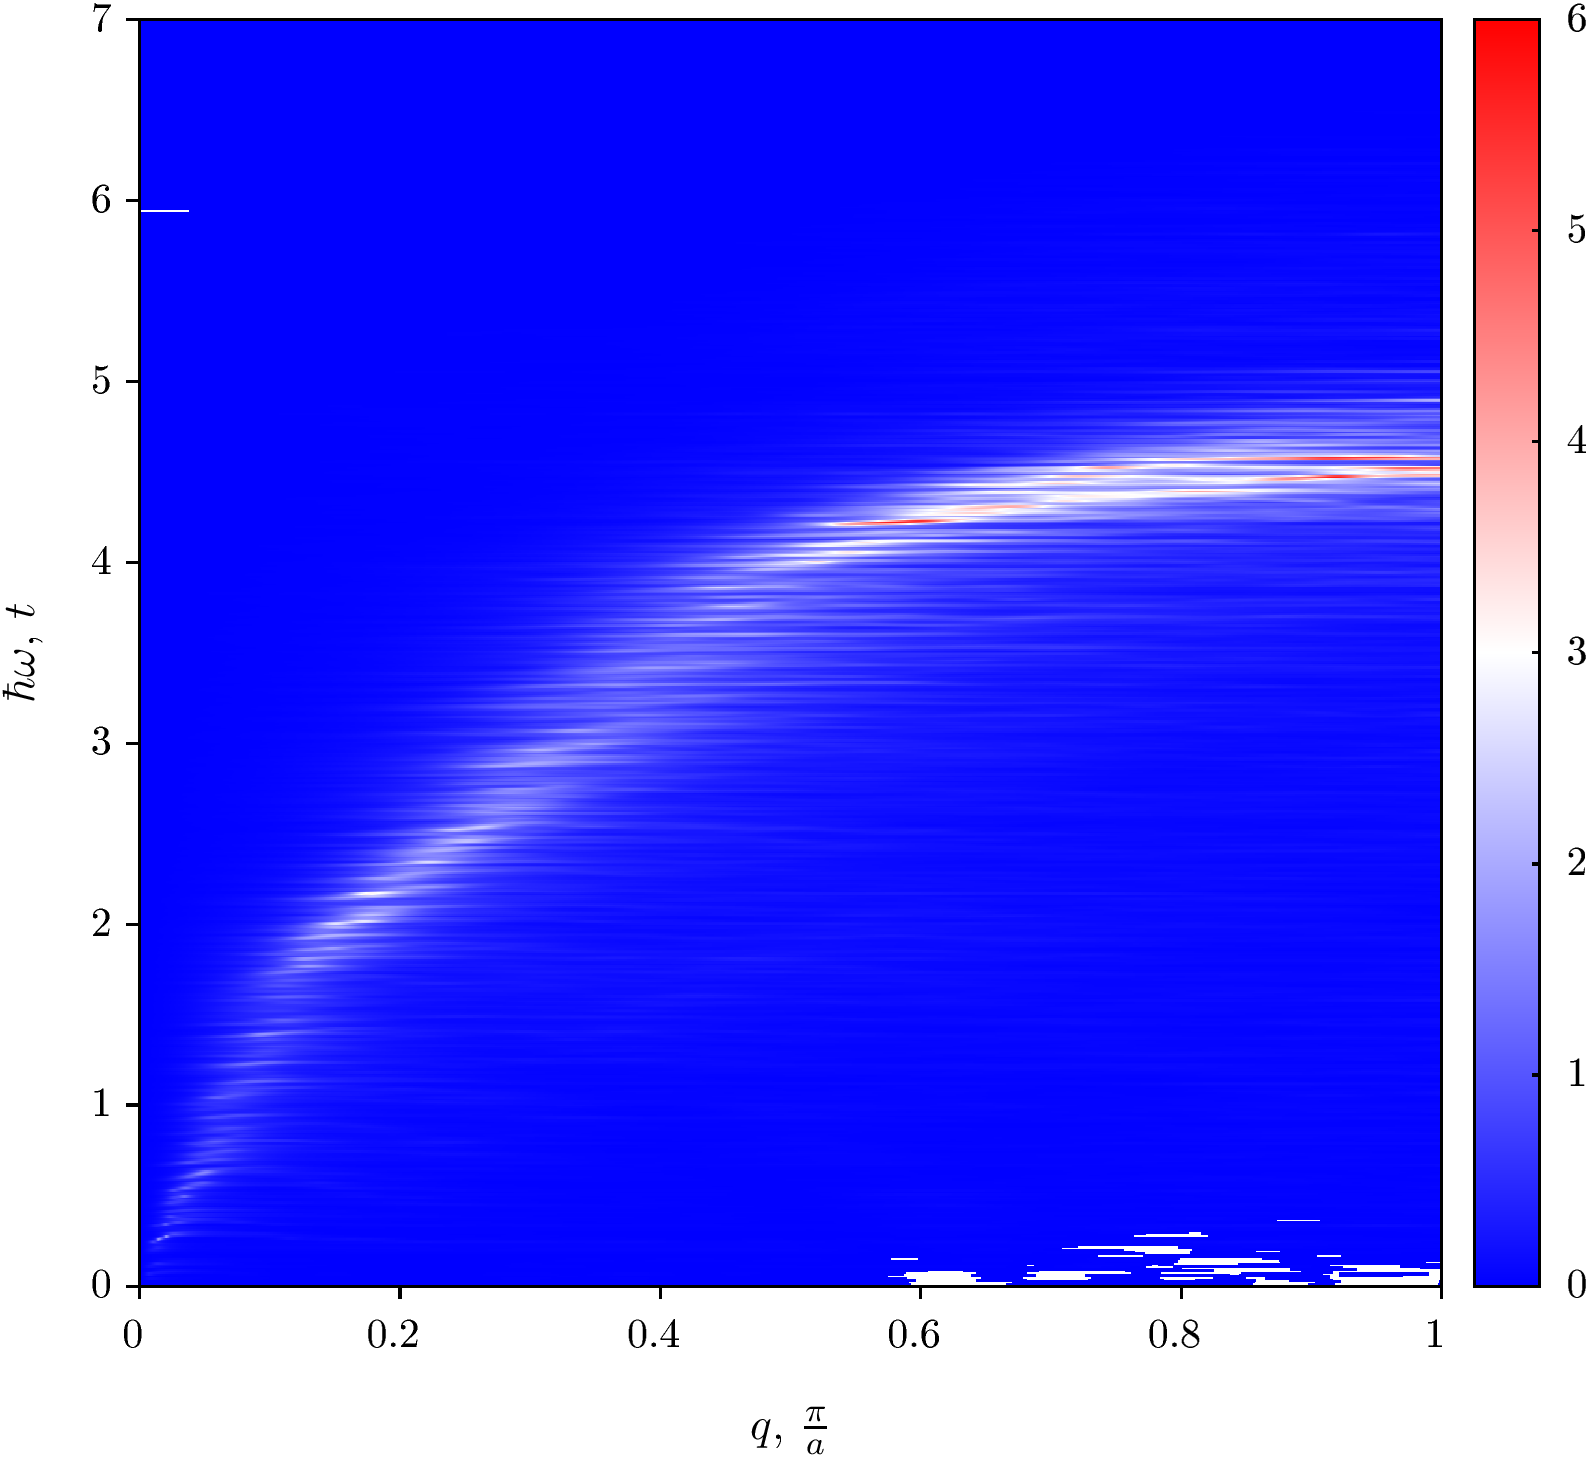
\includegraphics[width=\textwidth]{Spectrum-3rd-Q-Omega.png}
    \caption{Dispersion relation \ $-\operatorname{Im}[1 / \langle\mathbf{q}| \hat\varepsilon(\omega) |\mathbf{q}\rangle]$ for the third iteration Sierpinski carpet. $\mathbf{q}$ is chosen in the $x$ direction. There is some noise due to finite precision of numerical computations in the high momenta -- low energy regime. It does not interfere with the results, though.}
    \label{fig:spectrum-3rd-Q-Omega}
    \end{figure}

    We now turn to the results obtained in the $\mathbf{q}$--approach. Fig. \ref{fig:spectrum-3rd-Q-Omega} shows the loss function as function of both $\mathbf{q}$ and $\omega$. It is remarkable that there is such a close resemblance between this figure and the dispersion relation for a plain square sheet of the same size (fig. \ref{fig:spectrum-SL-Q-Omega}). Both curves look like a classical $\varepsilon(\omega) \propto \sqrt{q}$ dispersion relation for surface plasmons (see \cite{giuliani2005quantum}). It is quite fascinating, because fractals exhibit no translational invariance, i.e. $\mathbf{q}$ is not even a good quantum number. There is an interesting feature in the Sierpinski carpet's dispersion relation. The curve seems to be built from three almost straight segments. We are dealing with the third iteration of Sierpinski carpet. It means that there are three different sizes of ``holes''. The first segment corresponds to such long wavelengths that it ``does not notice'' the smaller holes, i.e. it acts as the first iteration fractal. The second segment corresponds to lower wavelengths, and second iteration holes begin to matter. And finally, third iteration holes come into play in the third segment. All these holes act like barriers in the $\mathbf{r}$--space, and result in some spread of the modes in the $\mathbf{q}$--space.

    \begin{figure}[h]
    \center
    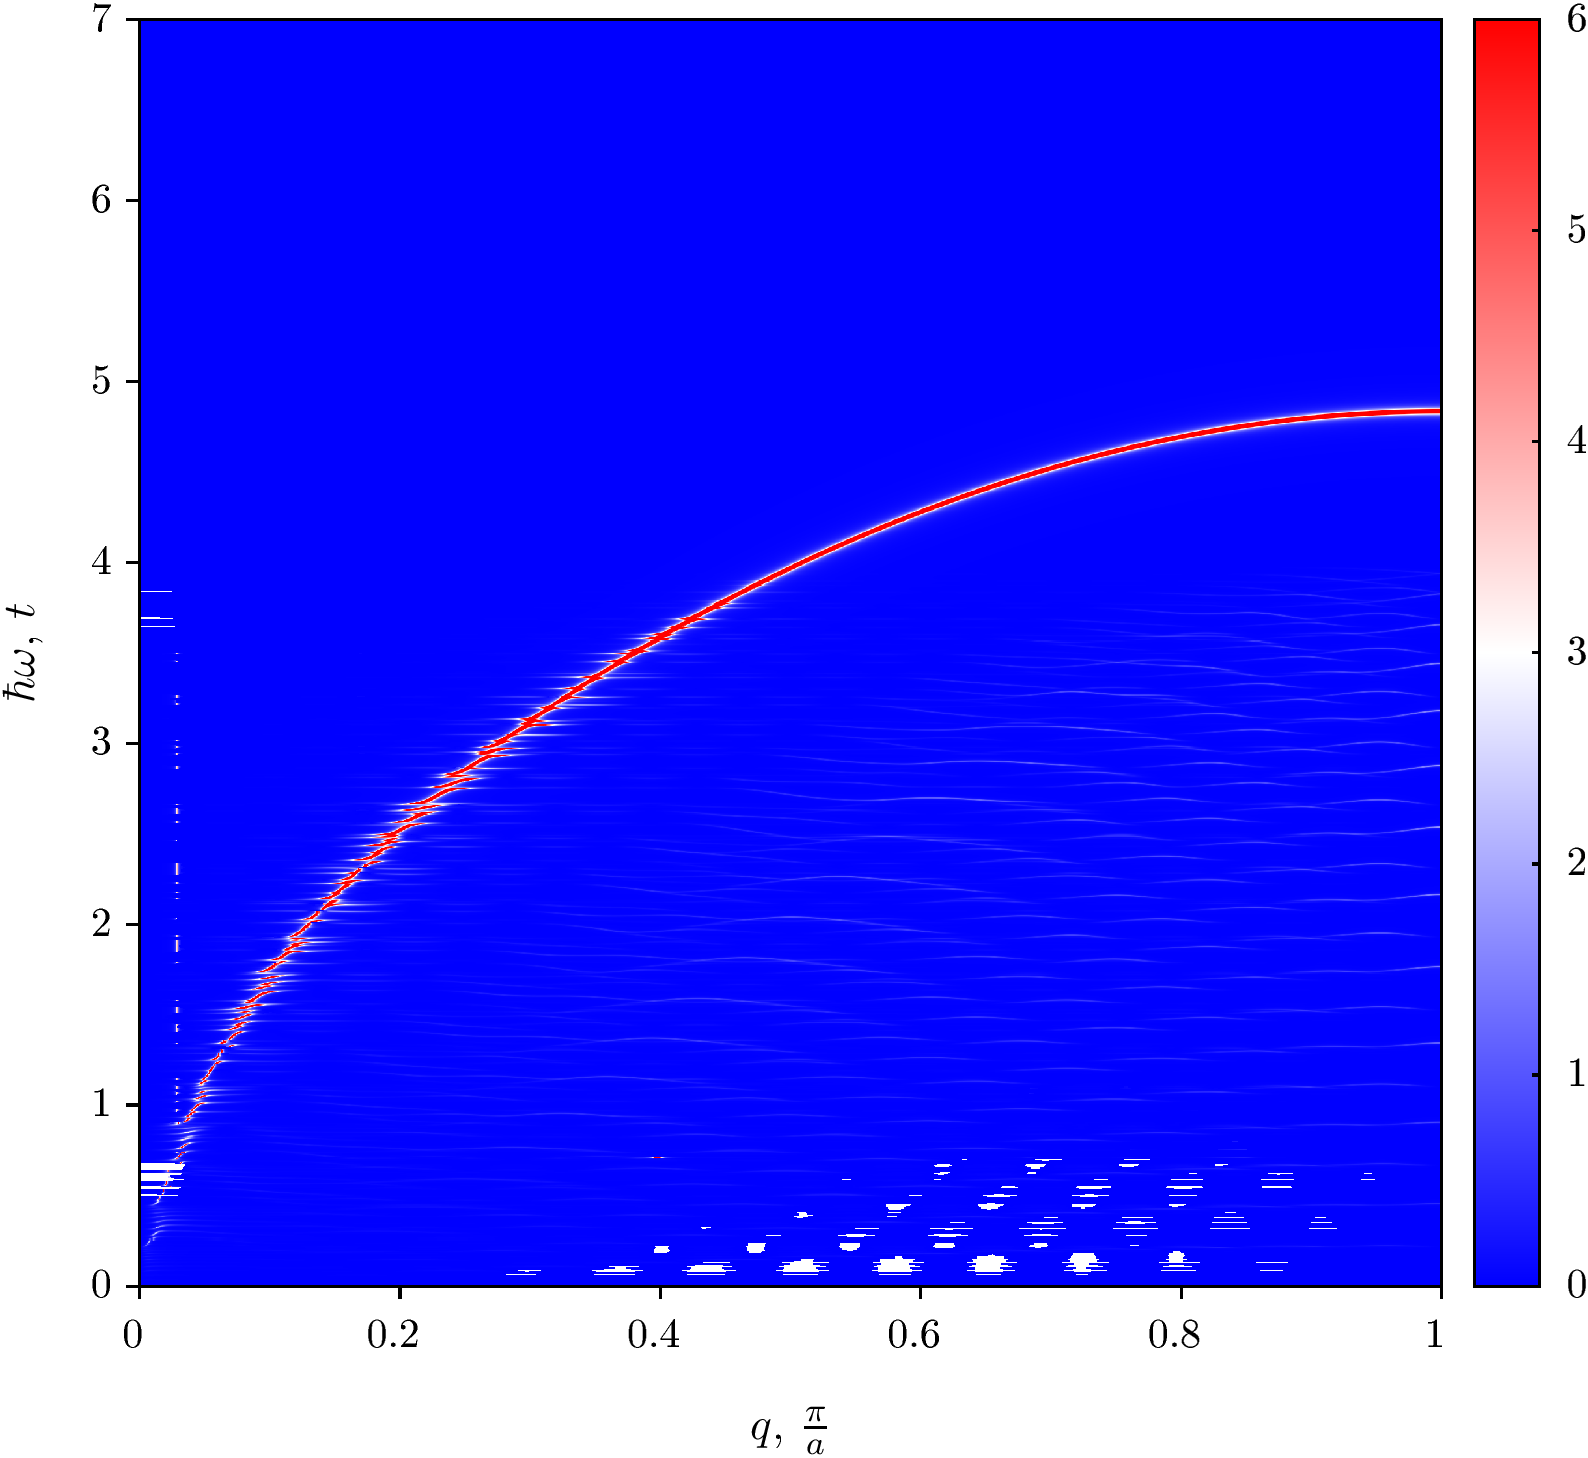
\includegraphics[width=\textwidth]{Spectrum-SL-Q-Omega.png}
    \caption{Dispersion relation \ $-\operatorname{Im}[1 / \langle\mathbf{q}| \hat\varepsilon(\omega) |\mathbf{q}\rangle]$ for the square lattice. $\mathbf{q}$ is chosen in the $x$ direction. Similarly to fig. \ref{fig:spectrum-3rd-Q-Omega} there is some noise due to finite precision of numerical computations.}
    \label{fig:spectrum-SL-Q-Omega}
    \end{figure}

\newpage
\section{Conclusion \& Outline}
    
    We have presented a new approach to calculating plasmonic properties of small systems. We have shown that it works. Although quite costly, with modern hardware this approach allows us to calculate the dielectric function of an arbitrary non-periodic lattice. We have also shown some first results obtained with this method, namely the fact that there are some well-defined plasmons in Sierpinski carpets. With current experimental techniques, these results can be proved experimentally.

    In the meantime, we hope to apply the method to other geometries. With the current implementation the maximum size of the system lies under a dozen thousands of sites. Modern GPUs have become extremely good (even better than CPUs) at matrix computations. There is thus a possibility of changing the underlying implementation of the method to make use of GPUs too in the hopes of speeding up the computations and allowing us to explore bigger systems.

\newpage
\appendix

\section{Code}
\label{code}

    As of now, there are \textit{no} open source projects that allow to perform $\mathbf{r}$--space calculations of plasmonic properties in the tight--binding approximation. We started a new project \cite{plasmon-cpp} to fill this gap. It uses \texttt{C++} as its primary language.

\begin{lstlisting}[mathescape]
    plasmon-cpp/
        bin/
            generate_system.py           $\Rightarrow$ hamiltonian generation script
            functions.sh                 $\Rightarrow$ data analysis utilities
        include/
            blas.hpp                     $\Rightarrow$ BLAS wrappers
            lapack.hpp                   $\Rightarrow$ LAPACK wrappers
            constants.hpp                $\Rightarrow$ physical constants
            dielectric_function_v2.hpp   $\Rightarrow$ calculation of $\hat\varepsilon$
        src/
            convert.cpp                  $\Rightarrow$ text $\leftrightarrow$ binary conversions
            hello.cpp                    $\Rightarrow$ calculation of $\hat\varepsilon(\omega)$
            potential.cpp                $\Rightarrow$ generation of $\hat V_\text{Coulomb}$
            solve_system.cpp             $\Rightarrow$ hamiltonian solver
\end{lstlisting}

    The project consists of three levels. The lowest layer provides wrappers around some of \texttt{BLAS} (\texttt{B}asic \texttt{L}inear \texttt{A}lgebra \texttt{S}ubprograms) and \texttt{LAPACK} (\texttt{L}inear \texttt{A}lgebra \texttt{Pack}age) routines. Currently only two realisations are supported: \texttt{ATLAS} \cite{atlas_siam} and \texttt{MKL} \cite{intel-mkl}. We plan to add support for GPU Computations later. The second layer implements eq. \eqref{eq:appl:result_w} using \texttt{MPI} (\texttt{M}essage \texttt{P}assing \texttt{I}nterface) to distribute the tasks between multiple nodes. The third layer consists of \texttt{Bash} scripts to allow for easy composition of tools and data analysis.

    Refer to the project page for further details.
 


\newpage
\bibliography{bibliography}

% \newpage
% \printindex

\end{document}
